\documentclass[11pt, a4paper]{article}


\usepackage{geometry}
\usepackage{layout}
\geometry{
  includeheadfoot,
  margin=2.54cm
}
\usepackage{amsmath}
\usepackage{amssymb}
\usepackage{amstext}
\usepackage{amsthm}
\usepackage{color}
\usepackage{framed}
\usepackage{url}
%\usepackage{showkeys}
%\usepackage{stmaryrd}
\usepackage{epsfig} 
\usepackage{graphicx} 
\usepackage{algorithmic}
\usepackage{algorithm}
\usepackage{type1cm}
%\usepackage{mathabx}
\usepackage{comment}

% Preprint version:
\includecomment{preprint}
\excludecomment{submitted}

% Submitted version:
%\excludecomment{preprint}
%\includecomment{submitted}


\renewcommand{\algorithmicrequire}{\bf Input:}
\renewcommand{\algorithmicensure}{\bf Output:}

\newcommand{\calA}{\mathcal{A}}
\newcommand{\calB}{\mathcal{B}}
\newcommand{\calC}{\mathcal{C}}
\newcommand{\calD}{\mathcal{D}}
\newcommand{\calE}{\mathcal{E}}
\newcommand{\calF}{\mathcal{F}}
\newcommand{\calG}{\mathcal{G}}
\newcommand{\calH}{\mathcal{H}}
\newcommand{\calK}{\mathcal{K}}
\newcommand{\calL}{\mathcal{L}}
\newcommand{\calM}{\mathcal{M}}
\newcommand{\calN}{\mathcal{N}}
\newcommand{\calO}{\mathcal{O}}
\newcommand{\calP}{\mathcal{P}}
\newcommand{\calQ}{\mathcal{Q}}
\newcommand{\calR}{\mathcal{R}}
\newcommand{\calS}{\mathcal{S}}
\newcommand{\calT}{\mathcal{T}}
\newcommand{\calU}{\mathcal{U}}
\newcommand{\calV}{\mathcal{V}}
\newcommand{\calW}{\mathcal{W}}
\newcommand{\calX}{\mathcal{X}}
\newcommand{\calY}{\mathcal{Y}}
\newcommand{\calZ}{\mathcal{Z}}

\newcommand{\frakI}{\mathfrak{I}}
\newcommand{\frakJ}{\mathfrak{J}}
\newcommand{\frakL}{\mathfrak{L}}
\newcommand{\F}{{\mathbb F}}
\newcommand{\R}{{\mathbb R}}
\newcommand{\C}{{\mathbb C}}
\newcommand{\N}{{\mathbb N}}
\newcommand{\htucker}{{\tt htucker}}
\newcommand{\epsrel}{{\epsilon_{\mathsf{rel}}}}
\newtheorem{theorem}{\bf Theorem}[section]
\newtheorem{definition}[theorem]{\bf Definition}
\newtheorem{lemma}[theorem]{\bf Lemma}
\newtheorem{example}[theorem]{\bf Example}
\newtheorem{remark}[theorem]{\bf Remark}
\newtheorem{notation}[theorem]{\bf Notation}
\newtheorem{corollary}[theorem]{\bf Corollary}
\newtheorem{proposition}[theorem]{\bf Proposition}
%\newcommand {\proof} {\par{\it Proof}. \ignorespaces}
%\newcommand {\eproof}
%      {\space
%        {\ \vbox{\hrule\hbox{\vrule height1.3ex\hskip0.8ex\vrule}\hrule}}
%        \par}

\newcommand{\vertical}[2]{\genfrac{}{}{0pt}{}{#1}{#2}}
%\newcommand{\qed}{\begin{flushright}$^\square$\end{flushright}}
\newcommand{\todo}[1]{\mbox{$$}\newline\textbf{\color{red}#1}\par}
\newcommand{\HTucker}{\mathcal H\text{-Tucker}}


\DeclareMathOperator{\vect}{vec}
\DeclareMathOperator{\rank}{rank}
\DeclareMathOperator{\diag}{diag}
\DeclareMathOperator*{\argmin}{arg\,min}
\DeclareMathOperator*{\argmax}{arg\,max}

% Norms
\newcommand{\norm}[1]{{\left\|#1\right\|}}
\newcommand{\norma}[1]{{\|#1\|}}
\newcommand{\normb}[1]{{\bigl\|#1\bigr\|}}
\newcommand{\normc}[1]{{\Bigl\|#1\Bigr\|}}
\newcommand{\normd}[1]{{\biggl\|#1\biggr\|}}
\newcommand{\norme}[1]{{\Biggl\|#1\Biggr\|}}

\newcommand{\innerprod}[2]{{\left\langle#1,#2\right\rangle}}
\newcommand{\innerproda}[2]{{\langle#1,#2\rangle}}
\newcommand{\innerprodb}[2]{{\bigl\langle#1,#2\bigr\rangle}}
\newcommand{\innerprodc}[2]{{\Bigl\langle#1,#2\Bigr\rangle}}
\newcommand{\innerprodd}[2]{{\biggl\langle#1,#2\biggr\rangle}}
\newcommand{\innerprode}[2]{{\Biggl\langle#1,#2\Biggr\rangle}}

\renewcommand{\tilde}{\widetilde}
\renewcommand{\hat}{\widehat}

\begin{document}

\title{{\tt htucker} --  A {\sc Matlab} toolbox for tensors in hierarchical Tucker format\thanks{Supported by the FNS research module \emph{Preconditioned methods
for large-scale model reduction} within the FNS ProDoc \emph{Efficient Numerical Methods for Partial Differential Equations}.}%
}

\author{\renewcommand{\thefootnote}{\arabic{footnote}}Daniel Kressner\footnotemark[1] \and \renewcommand{\thefootnote}{\arabic{footnote}}Christine Tobler\footnotemark[1]}

\footnotetext[1]{Chair of Numerical Algorithms and HPC, MATHICSE, EPF Lausanne, CH-1015 Lausanne, Switzerland. \{daniel.kressner,christine.tobler\}@epfl.ch}

%\footnotetext[2]{Seminar for Applied Mathematics, D-MATH, ETH Zurich, CH-8092 Zurich. ctobler@math.ethz.ch}



\maketitle

\begin{preprint}                                                                                                                               
$\ $ \\[-1cm]
\begin{center}
\Large -- Extended version -- 
\end{center}
\end{preprint}

\begin{abstract}
The hierarchical Tucker format is a storage-efficient scheme to approximate and represent
tensors of possibly high order. This paper presents a {\sc Matlab} toolbox, along with
the underlying methodology and algorithms, which provides a convenient way to work with this format. The toolbox not only allows for the efficient storage and manipulation of tensors in hierarchical Tucker format
but also offers a set of tools for the development of higher-level algorithms.
Several examples for the use of the toolbox are given.
%This includes simple algorithms, such as an iterative method for orthogonalizing tensors, as well as more complex applications, such as the solution of parameter-dependent elliptic partial differential equations.
\end{abstract}
%\tableofcontents

\section{Introduction}

A \emph{tensor} $\calX \in \C^{n_1\times n_2\times\cdots \times n_d}$ with $n_1,\ldots,n_d\in \N$ is a $d$-dimensional array with entries $\calX_{i_1 i_2 \cdots i_d} \in \C$. Usually,
$d$ is called the \emph{order} of the tensor and the focus of this paper is on tensors of higher 
order, say, $d = 5$ or $d = 10$ or even $d = 100$. A typical scenario is that $\calX$ represents a $d$-variate function $f: [0,1]^d \to \C$ sampled on a tensor grid or approximated in a tensorized basis.

It is in general impossible to store a higher-order tensor explicitly, simply because
the number of entries grows exponentially with $d$.
Various data-sparse formats have been developed to address this issue. Depending on the application,
these formats may allow for the approximate representation and manipulation of a tensor under dramatically
reduced storage and computing requirements. For example, consider the approximation of $\calX$ by
a rank-$1$ tensor:
\begin{equation} \label{eq:tensorrank1}
 \vect(\calX) \approx u_d \otimes u_{d-1} \otimes \cdots \otimes u_1, \qquad u_1 \in \C^{n_1},\ \ldots,\ u_d \in \C^{n_d},
\end{equation}
where $\vect$ stacks the entries of a tensor in reverse lexicographical order
into a long column vector and $\otimes$ denotes the standard Kronecker product. Then, instead of the $n_1\cdot n_2 \cdots n_d$ entries of $\calX$, only the $n_1+n_2+\cdots+n_d$ entries of $u_1,\ldots,u_d$ need to be stored.
On the function level, this corresponds to an approximation of $f$ by a separable function.

A typical application we have in mind is when $\calX$ arises from the discretization
of a high-dimensional or parameter-dependent partial differential equation and is only given implicitly
as the solution to a typically huge (non)linear system or eigenvalue problem. There are two quite different
strategies to employ a data-sparse format for the solution of such problems. The more straightforward
one is to apply a standard iterative method, e.g., a conjugate gradient method, and approximate each iterate in the data-sparse format.
For this purpose, it is desirable to keep the approximation error negligible; otherwise the accuracy and convergence of the method may be compromised. Examples for this strategy can be found in~\cite{BalG10,HacKST08,KhoO10,KhoS10,KreT10b}.
The second strategy is to reformulate the problem at hand as an optimization problem with the admissible set of solutions
restricted to data-sparse tensors, see~\cite{Espig2012e,HolRS10b,Huckle2013,KocL10,OseK10,Sch11} and the references therein.  Beyond these two main strategies, there exist further approaches tailored to particularly structured problems, see, e.g.,~\cite{Gra04a,KreT10}. While the mathematical understanding is still somewhat limited, there is strong numerical evidence that such data-sparse algorithms can handle a wide variety of problems that are far from tractable by classical numerical methods. 

In most applications, it is unlikely that a rank-$1$ representation~(\ref{eq:tensorrank1}) yields a satisfactory
approximation error. This can be improved by considering the more general CP (Canonical Polyadic) decomposition \cite{Har70,CarC70}
\begin{equation} \label{eq:cp}
 \vect(\calX) \approx \sum_{j = 1}^R u^{(j)}_d \otimes u^{(j)}_{d-1} \otimes \cdots \otimes u^{(j)}_1, \qquad u^{(j)}_1 \in \C^{n_1},\ \ldots,\ u^{(j)}_d \in \C^{n_d},
\end{equation}
which still requires little memory, provided that $R$ does not become too large. Unfortunately,
developing a robust and efficient algorithm for this format, which yields an approximation to any desirable accuracy,
remains a subtle problem, see~\cite{AcaDK11,Espig2012d} for recent progress.
This problem is much less subtle for the Tucker decomposition \cite{Tucker66},
\begin{equation} \label{eq:tucker}
 \vect(\calX) \approx \big( U_d \otimes U_{d-1} \otimes \cdots \otimes U_1 \big) \vect(\calC), \qquad U_1 \in \C^{n_1\times r_1}, \ \ldots,\ U_d \in \C^{n_d\times r_d},
\end{equation}
with the so called core tensor $\calC\in \C^{r_1\times r_2 \times \cdots \times r_d}$.
The HOSVD (Higher-Order SVD)~\cite{DeLDV00} provides a simple, nearly optimal solution to the approximation
problem~(\ref{eq:tucker}). However, the need for storing $\calC$ still results in memory requirements that grow exponentially with $d$.

Motivated by the limitations of the two classical decompositions~(\ref{eq:cp}) and (\ref{eq:tucker}),
various other decompositions have been developed in the numerical analysis community with the aim
of combining the advantages of both. This includes the tensor train decomposition~\cite{KhoO09},
the closely related but somewhat more general HTD (hierarchical Tucker decomposition)~\cite{Gra10,HacK09}, and even more general tensor networks \cite{EspHHS11}.
In the computational physics community, matrix product states and tensor networks play a central role
in DMRG (density matrix renormalization group) techniques for computing ground states of quantum many-body systems, see~\cite{Sch11} for an introduction.
In the case of tensors that contain values of a multivariate function, additional properties inherited from the regularity of the function can in certain cases lead to a
significantly higher compression in HTD (and related decompositions) compared to Tucker, see, e.g.,~\cite{Hac12} for such a discussion.

% \textcolor{red}{ The lower storage requirements of the HTD
%   decompositions come at the price of additional requirements on the
%   tensor. However, in the case of tensors that contain values of a
%   multivariate function, additional properties inherited from the
%   regularity of the function can in certain cases lead to a
%   significantly higher compression in HT decomposition compared to the
%   Tucker decomposition. This is the case, for example, for any
%   function that can be well approximated using sparse grids
%   \cite[Sec.11.6]{Hac12}, and for the functions in
%   Section~\ref{sec:examples}.}

Existing {\sc Matlab} toolboxes for working with low-rank tensor formats are the 
N-way toolbox by Andersson and Bro~\cite{AndB00}, the Tensor Toolbox by Bader and Kolda~\cite{BadK06,BadK07}, as well as the TT-Toolbox by Oseledets~\cite{tttoolbox,Osel09}.
TensorCalculus~\cite{tensorcalculus} is a C++ library for more general tensor networks.
In computational physics, a number of related software packages have been developed
in the context of DMRG techniques for simulating quantum networks, see, e.g.,~\cite{Bau11}.

The main goal of this paper is to provide a convenient framework for
the development and implementation of algorithms based on the
hierarchical Tucker decomposition. In particular, methods for the
truncation of a given tensor to HTD, i.e., the approximation by a
low-rank tensor in HTD, are implemented and discussed in
Section~\ref{sec:truncation}.
A set of advanced tools allows for the development of higher-level algorithms.
Moreover, this work contains a number of new contributions:
\begin{itemize}
\item Efficient algorithms for HTD tensor-tensor contraction, including the inner product
between two tensors, are given in Sections~\ref{sec:generalcontraction} and~\ref{sec:reducedgramians}.
 \item A new variant of truncation to HTD without initial orthogonalization
is presented in Section~\ref{sec:trunc_var} and demonstrated to result in an efficient and numerically 
robust way for adding tensors in Section~\ref{sec:addtruncate}.
%\item Various bounds for the truncation error have been given, partly new and partly improving an existing one.
\item New algorithms for exact and approximate elementwise multiplication of tensors in HTD are presented in Section~\ref{sec:elementwise}.
\item A framework for representing linear operators in HTD is presented in Section~\ref{sec:linop}
and an explicit representation for a discretized Laplace operator has been given.
\end{itemize}
All our algorithms are mainly based on calls to level 3 BLAS and LAPACK functionality. 

The rest of this paper is organized as follows.
Section~\ref{sec:preliminaries} introduces basic tools for working
with tensors as well as the HTD.
%Note that we will only briefly introduce the concepts needed in this
%paper and refer the reader to~\cite{Hac12,KolB09} for more
%comprehensive introductions to tensor computations.
In Section~\ref{sec:basicfunctionality}, we
describe the basic functionality and data structures of our {\sc
  Matlab} toolbox \htucker.  Section~\ref{sec:basicops} is concerned
with basic operations on tensors in HTD, such as $\mu$-mode matrix
products and orthogonalization, and their implementation in \htucker.
Tensor-tensor contractions are discussed in
Section~\ref{sec:contraction}, including, e.g., inner products.  In
Section~\ref{sec:truncation}, we present several methods for
approximating a tensor either given explicitly or given in HTD by a
tensor in HTD (of lower rank). Section~\ref{sec:elementwise} is
concerned with elementwise multiplication, and
Section~\ref{sec:linop} with the representation 
of linear operators on tensors in HTD.  Finally,
several examples for working with \htucker{} are given in
Section~\ref{sec:examples} %
\begin{submitted}

Examples for working with \htucker{} and a list of its complete functionality can be found in
the preprint~\cite{KreT11tr}, an extended version of this manuscript.
%Section~\ref{sec:examples}% xamples and An extended version of this paper containing  preprint
\end{submitted}
\begin{preprint}
  and a list of the complete functionality of \htucker{} can be found
  in Appendix~\ref{sec:functionality}, while proofs of some of the
  error bounds given in Section~\ref{sec:truncation} can be found in Appendix~\ref{sec:proofs}.
\end{preprint}



\section{Preliminaries} \label{sec:preliminaries}

This section summarizes the mathematical foundation of the hierarchical Tucker decomposition (HTD) 
and our {\sc Matlab} toolbox.
Necessary tensor concepts will be briefly introduced.  We
refer the reader to the survey paper~\cite{KolB09} and to the book~\cite{Hac12}
for a more comprehensive introduction.


\subsection{Matricization and HOSVD} \label{sec:hosvd}

To understand the principles behind HTD, it is helpful to recall the matricization and HOSVD of tensors.
A tensor $\calX \in \C^{n_1\times n_2\times\cdots \times n_d}$ has $d$ different \emph{modes} $1,\ldots,d$.
Consider a splitting of these modes into two disjoint sets:
$\{1,\ldots,d\}  = t\cup s$ with $t = \{t_1,\ldots,t_k\}$ and $s = \{s_1,\ldots,s_{d-k}\}$.
Then the corresponding \emph{matricization} of these modes is obtained by
merging the first group into row indices and the second group into column indices:
\[
 X^{(t)} \in \C^{(n_{t_1}\cdots n_{t_k}) \times (n_{s_1}\cdots n_{s_{d-k}})} \quad \text{with}
\quad \left( X^{(t)} \right)_{(i_{t_1},\ldots,i_{t_k}),(i_{s_1},\ldots,i_{s_{d-k}})} := \calX_{i_1,\ldots,i_d}
\]
for any indices $i_1,\ldots,i_d$ in the multi-index set $\{1,\ldots,n_1\}\times \cdots \times \{1,\ldots,n_d\}$.
Of course, the order in which the indices are merged is important.
In the following, we assume reverse lexicographical order of the multi-indices but any other consistently employed order would be suitable.
Note that the matricization is \emph{not} independent of the ordering of the modes
$t_1,\ldots,t_k$ and $s_1,\ldots,s_{d-k}$ in the sets $t$ and $s$, respectively. If not
noted otherwise, we assume the modes to be in increasing order.

%In the extreme case, $X^{(\{1,\ldots,d\})}$ corresponds to the column vector $\vect(\calX)$.
\begin{preprint}
\begin{figure}
 \begin{center}
  \begin{minipage}{0.3\textwidth}
\begin{center}
   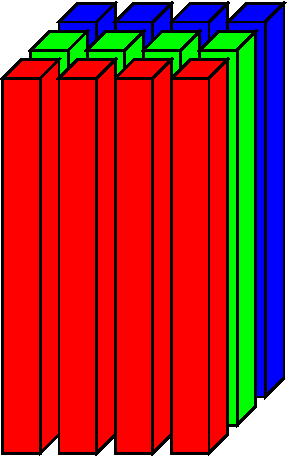
\epsfig{file = tensormode1, scale = 0.2} \\
$\calX$  \\[0.2cm]
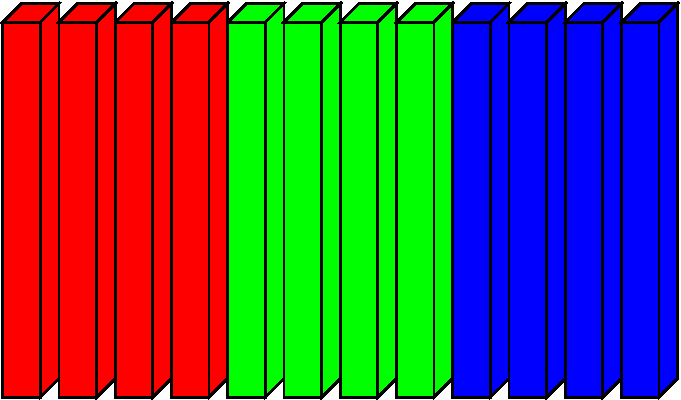
\epsfig{file = tensormode2, scale = 0.2}  \\
$X^{(\{1\})}$ 
\end{center}
  \end{minipage}$\quad$
\begin{minipage}{0.3\textwidth}
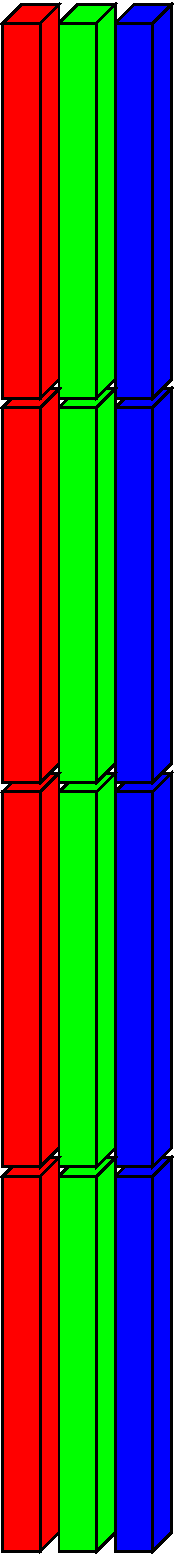
\epsfig{file = tensormode3, scale = 0.2}  \\ 
$X^{(\{1,2\})}$ 
\end{minipage}
 \end{center}
\caption{Illustration of an $n_1\times 4 \times 3$ tensor $\calX$ with matricizations $X^{(\{1\})}$ and $X^{(\{1,2\})}$.}
\end{figure}
\end{preprint}

As a special case, consider the so called $\mu$-mode matricization \[
X^{(\mu)} \in \C^{n_\mu \times (n_1\cdots n_{\mu-1} n_{\mu+1} \cdots n_{d})}, \qquad \mu = 1,\ldots,d.
\]
Then the tuple $(r_1,\ldots,r_d)$ with $r_\mu = \text{rank} \big( X^{(\mu)} \big)$ is called
the \emph{multilinear rank} of $\calX$. To obtain an approximation of lower 
multilinear rank $(\tilde r_1,\ldots,\tilde r_d)$, with $\tilde r_\mu \le r_\mu \le n_\mu$, we let $U_\mu \in \C^{n_\mu \times \tilde r_\mu}$ contain
the $\tilde r_\mu$ dominant left singular vectors of $X^{(\mu)}$, which can be obtained, e.g., from a truncated SVD $X^{(\mu)} \approx U_\mu \Sigma_\mu V_\mu^H$. Then the HOSVD takes the form of a Tucker decomposition
\begin{equation} \label{eq:hosvd}
 \vect(\calX) \approx \vect(\tilde \calX) := (U_d \otimes \cdots \otimes U_1) \vect(\calC),
\end{equation}
with the core tensor \[
\vect(\calC) := (U^H_d \otimes \cdots \otimes U^H_1) \vect(\calX) \in \C^{\tilde r_1\times \cdots \times \tilde r_d}.
\]
This choice of $\calC$ minimizes $\| \calX - \tilde \calX \|_2$
for given $U_1, \ldots, U_d$ with orthonormal columns. Here and in the following, $\|\calY\|_2$ denotes the Euclidean norm of the vectorization: $\|\calY\|_2 = \|\vect(\calY)\|_2$. An important feature of the HOSVD, it can be shown~\cite{DeLDV00} that the obtained approximation is nearly optimal among \emph{all} tensors of multilinear rank $(\tilde r_1,\ldots,\tilde r_d)$ or lower:
\begin{equation} \label{eq:hosvdbestapprox}
 \| \calX - \tilde \calX \|_2 \le \sqrt{d} \cdot \inf \big\{ \|\calX - \calY\|_2:\ \text{rank}(Y^{(\mu)}) \le \tilde r_\mu,\ \mu = 1,\ldots, d \big\}.
\end{equation}

\subsection{The Hierarchical Tucker Decomposition (HTD)}

In contrast to the Tucker decomposition, HTD employs a
hierarchy of matricizations, motivated by the following nestedness property.
Note that our use of the symbol $\subset$ for set inclusion allows for equal sets.
\begin{lemma}[{\cite[Lemma 17]{Gra10summer}}] \label{lemma:nested}
 Let $\calX \in \C^{n_1\times \cdots \times n_d}$ and $t = t_l\cup t_r$ for $t_l = \{i_l, i_l+1, \ldots, i_m\}$ and $t_r = \{i_m+1, \ldots, i_r\}$. Then $\text{\rm span}\big(X^{(t)}\big)\subset \text{\rm span}\big(X^{(t_r)} \otimes X^{(t_l)}\big)$.
\end{lemma}
\begin{proof}
Any column of $X^{(t)} = X^{(i_l,\ldots,i_r)}$ can be considered as the vectorization of a tensor $\calC \in 
\C^{n_{i_l}\times \cdots \times n_{i_r}}$. The columns of the matricization $C^{(t_l)}$ are
clearly contained in $\text{span}\big(X^{(t_l)}\big)$ and hence
\[
 C^{(t_l)} = X^{(t_l)} \big(X^{(t_l)}\big)^+ C^{(t_l)},
\]
where $M^+$ denotes the Moore-Penrose pseudoinverse of a matrix $M$. Analogously,
\[
 \big( C^{(t_l)} \big)^T = C^{(t_r)} = X^{(t_r)} \big(X^{(t_r)}\big)^+ C^{(t_r)}.
\]
These two relations imply \[
C^{(t_l)} =  X^{(t_l)} \underbrace{\Big( \big(X^{(t_l)}\big)^+ C^{(t_l)}  \big(X^{(t_r)}\big)^{+T} \Big)}_{=:V} \big(X^{(t_r)}\big)^{T}
\ \Rightarrow\ 
\vect(\calC) = \big(X^{(t_r)} \otimes X^{(t_l)}\big) \vect(V).
\]
\end{proof}
\noindent Given any bases $U_t,U_{t_l},U_{t_r}$ for the column spaces
of $X^{(t)}, X^{(t_l)}, X^{(t_r)}$, the result of
Lemma~\ref{lemma:nested} implies the existence of a so called transfer
matrix $B_t$ such that
\begin{equation} \label{eq:nestedmatrix}
 U_t = (U_{t_r} \otimes U_{t_l}) B_t, \quad B_t \in \C^{r_{t_l} r_{t_r} \times r_t},
\end{equation}
where $r_t, r_{t_l},r_{t_r}$ denote the ranks of the corresponding
matricizations. Applying this relation recursively, until $t_l$ and
$t_r$ become singletons, leads to the HTD.
\begin{example} \label{example:d4} Repeated application of~(\ref{eq:nestedmatrix}) for $d = 4$:
\begin{eqnarray}
 \text{vec}(\calX) = X^{(\{1,2,3,4\})} &=& (U_{34} \otimes U_{12}) B_{1234} \nonumber \\
 U_{12} &=& (U_2\otimes U_1) B_{12} \nonumber \\
 U_{34} &=& (U_4\otimes U_3) B_{34} \nonumber \\
\Rightarrow \quad {\text{vec}(\calX)} &{=} &
{(U_4\otimes U_3  \otimes U_2\otimes U_1) (B_{34}\otimes B_{12})  B_{1234}}. \label{eq:HTD4}
\end{eqnarray}
It is often advantageous to reshape the transfer matrices:
\begin{eqnarray*}
B_{1234} \in \C^{r_{12}r_{34}\times 1} & \Rightarrow &  \calB_{1234} \in \C^{r_{12}\times r_{34} \times 1}, \\
 B_{12} \in \C^{r_1r_2\times r_{12}} & \Rightarrow & \calB_{12} \in \C^{r_1\times r_2\times r_{12}}, \\
 B_{34} \in \C^{r_3r_4\times r_{34}} & \Rightarrow &  \calB_{34} \in \C^{r_3\times r_4\times r_{34}}. 
\end{eqnarray*}
To avoid cluttering the notation we write $B_{12}$ instead of $B_{\{1,2\}}$,
$U_{12}$ instead of $U_{\{1,2\}}$, $r_{12}$ instead of $r_{\{1,2\}}$,
and so on.

An illustration of the hierarchical structure and the data to be stored for the HTD~(\ref{eq:HTD4})
is given in Figure~\ref{fig:order4tensor}.
\end{example}
\begin{figure}
\begin{center}
  \resizebox{4.5cm}{!}{\input dim_tree.eps_t}
  $\qquad\qquad \qquad$
  \resizebox{4cm}{!}{\input htensor_dimtree.pdf_t}
\end{center}
\caption{Illustration of the HTD~(\ref{eq:HTD4}) for $d = 4$.} \label{fig:order4tensor}
\end{figure}

The general construction of an HTD requires a hierarchical splitting of the modes $1,\ldots,d$.
\begin{definition}
 A binary tree $\calT$ with each node represented by a subset of $\{1,\ldots,d\}$ is called a \emph{dimension tree} if 
 the root node is $\{1,\ldots,d\}$, each leaf node is a singleton, and each parent node is the disjoint union of its two children. 
In the following, we denote:
\begin{center}
\begin{tabular}{rl}
$\calL(\calT)$ & set of all leaf nodes; \\
$\calN(\calT)$ & set of all non-leaf nodes, $\calN(\calT) = \calT \setminus \calL(\calT)$. 
\end{tabular}
\end{center}
\end{definition}
\begin{remark}
 For convenience of notation, we impose the following additional
 assumption on the left and right children $t_l,t_r$ of a node $t$ in
 the dimension tree: Each element of $t_l$ is smaller than any element
 of $t_r$. Note that this assumption can always be satisfied by an
 appropriate reordering of the modes.
\end{remark}
It is not hard to see that the number of non-leaf nodes is always
$d-1$.  An example of a dimension tree is given in
Figure~\ref{fig:dimtree}.
\begin{figure}
\begin{center}
  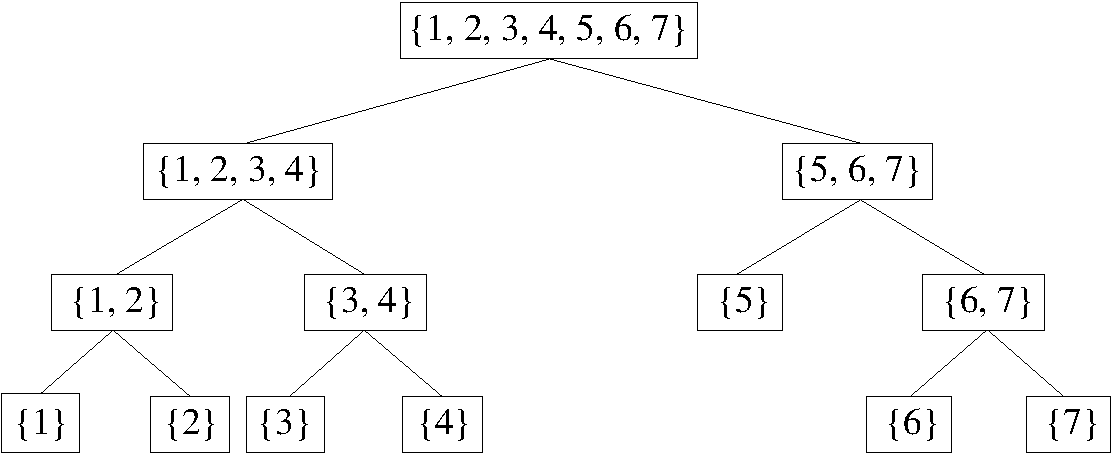
\includegraphics[width=10cm]{dimtree_7.pdf}
\end{center}
\caption{A dimension tree for $d = 7$.} \label{fig:dimtree}
\end{figure}

Having prescribed a maximal rank $k_t$ for each node $t \in \calT$, the set of \emph{hierarchical Tucker tensors of
hierarchical rank at most $(k_t)_{t\in\calT}$} is defined as
\[
 \HTucker\big( (k_t)_{t\in\calT} \big) = \Big\{ \calX \in \C^{n_1\times\cdots\times n_d}:\,\text{rank}\big(
X^{(t)} \big) \le k_t \text{ for all } t\in \calT
\Big\}.
\]
Such a hierarchical Tucker tensor $\calX$ is stored in the \emph{hierarchical Tucker format} as follows.
At each leaf node $\{\mu\}$ a basis $U_{\mu} \in \C^{n_\mu \times r_\mu}$, where
$r_\mu := \text{rank}\big(X^{(\mu)}\big) \le k_\mu$, is stored.
At each parent node $t$ with children $t_l$ and $t_r$, the third-order transfer tensor $\calB_t \in \C^{r_{t_l} \times r_{t_r} \times r_t}$ satisfying~(\ref{eq:nestedmatrix}) with $B_t \equiv B_t^{(\{1,2\})}$ is stored. Equivalently,~(\ref{eq:nestedmatrix}) can be written as
\begin{equation} \label{eq:generalrecursion}
(U_t)_{:,q} = \sum_{i=1}^{r_{t_l}} \sum_{j=1}^{r_{t_r}}
\Big( (U_{t_r})_{:, j} \otimes (U_{t_l})_{:, i} \Big)
(\calB_t)_{i, j, q}, \quad q = 1,2,\ldots,r_t. 
\end{equation}
The HTD for $\calX$ is obtained by recursively inserting~(\ref{eq:nestedmatrix}) as illustrated in
Example~\ref{example:d4}.

In summary, the hierarchical Tucker format is represented by $d$ matrices $U_\mu$ and $(d-1)$
transfer tensors $\calB_t$. 
Hence, if $r = \max\{r_t:\,t\in \calT \}$ and $n = \max\{n_1,\ldots,n_d\}$, the storage
requirements are bounded by
\begin{equation} \label{eq:complexity}
 dnr + (d-2) r^3 + r^2,
\end{equation}
where we have used that the transfer tensor at the root can actually be considered as a matrix of size at most $r\times r$. While the complexity bound~\eqref{eq:complexity} appears to indicate linear dependence in $d$, it is important to note that such a conclusion only
holds when the maximal hierarchical rank $r$ can be assumed to stay constant as $d$ increases. This is a rather strong assumption that is satisfied only in specific applications.

\section{Basic Functionality of the Toolbox} \label{sec:basicfunctionality}

To conveniently work with tensors in HTD, we have implemented a new {\sc Matlab}
class {\tt htensor}, inspired by the classes {\tt ktensor} (for tensors in CP decomposition)
and {\tt ttensor} (for tensors in Tucker decomposition) available in the Tensor Toolbox~\cite{BadK06}. 
In the following, we describe the structure of {\tt htensor} as well as its
basic functionality.

\subsection{Fields and properties of {\tt htensor}} \label{sec:classhtensor}

An instance of {\tt htensor} contains two arrays specifying the dimension tree, an orthogonalization flag,
as well as the matrices and transfer tensors representing an HTD corresponding to
this dimension tree.

Each node of the dimension tree is associated with an index $i \in \{1,\ldots,2d-1\}$, such that each child node 
has a larger index than the parent node.
Consequently, the root node has index~$1$. The $(2d-1)\times 2$ integer array {\tt children}
specifies the structure of the dimension tree as follows: \texttt{children(i, 1)} is the left child of node $i$, and
\texttt{children(i, 2)} is the right child of node $i$. Both entries are zero if node $i$ is a leaf node.
The $1 \times d$ integer array \texttt{dim2ind} gives the index
of the leaf node associated with each mode $\mu=1, \ldots, d$.
%The cell array \texttt{dims} contains the dimensions represented by each
%node. For a leaf node $i$, \texttt{dims\{i\}} is just a scalar 
%and for any other node $i$, we have
%\texttt{dims\{i\} = [dims\{children(i, 1)\}, dims\{children(i, 2)\}]}.
The matrices $U_t$ and transfer tensors $B_t$ are stored in the cell
arrays \texttt{U} and \texttt{B}, respectively. Note that \texttt{U\{i\}} is a matrix if
\texttt{i} is a leaf node and an empty array for any other node.
Finally, the boolean flag \texttt{is\_orthog} indicates whether the HTD is
orthogonalized, see Section~\ref{sec:orthogonalization}.
%
\begin{framed}\noindent
\textbf{\texttt{htensor} for $d = 4$ (see also Example~\ref{example:d4}):}\\
\vspace{-3ex} 
%x.dims: {[1 2 3 4], [1 2], [3 4], 1, 2, 3, 4}
\begin{verbatim}
x.children: [2, 3; 4, 5; 6, 7; 0, 0; 0, 0; 0, 0; 0, 0]
x.dim2ind: [4 5 6 7]
x.U: {[] [] [] [4x4 double] [5x4 double] [6x6 double] [7x3 double]}
x.B: {[4x5 double] [4x4x4 double] [6x3x5 double] [] [] [] []}
x.is_orthog: false
\end{verbatim}
\end{framed}
\begin{preprint}
Apart from the fields defining the HTD, {\tt htensor} has additional fields
for accessing frequently required properties.
\begin{framed}\noindent 
\textbf{Properties of \texttt{htensor}:}\\
\begin{tabular}{ll}
\texttt{x.nr\_nodes} & number of nodes in the dimension tree.\\
\texttt{x.parent(i)} & returns the index of the parent of node $i$.\\
\texttt{x.sibling(i)} & returns the index of the sibling of node $i$.\\
\texttt{x.is\_leaf(i)} & true if node $i$ is a leaf node.\\
\texttt{x.is\_left(i)} & true if node $i$ is a left child.\\
\texttt{x.is\_right(i)} & true if node $i$ is a right child.\\
\texttt{x.lvl(i)} & level of node $i$ (distance from root node).\\
\texttt{x.dims\{i\}} & modes represented by node $i$.\\
\texttt{x.bin\_dims(i, :)} & modes represented by node $i$ (logical array).\\
\texttt{x.rank(i)} & hierarchical rank at node $i$.\\
\end{tabular}
\end{framed}
\end{preprint}
\subsection{Constructors of {\tt htensor}} \label{sec:constructor}
%
There are several ways to construct an \texttt{htensor} instance. In the following,
we only illustrate the most common ways and refer to the documentation, e.g., {\tt help htensor/htensor},
for more details. 
\begin{framed}
\noindent \textbf{Examples for constructors of \texttt{htensor}:}\\
\texttt{x = htensor([4 5 6 7])} constructs a zero \texttt{htensor} of size $4 \times 5 \times 6 \times 7$.\\
\texttt{x = htensor([4 5 6 7], 'TT')} constructs a zero \texttt{htensor} of size $4 \times 5 \times 6 \times 7$, with a degenerate, TT-like dimension tree.\\
\texttt{x = htensor(\{U1, U2, U3\})} constructs an \texttt{htensor} from the CP tensor defined by $\calX(i_1, i_2, i_3) = \sum_{j=1}^R U_1(i_1, j) U_2(i_2, j) U_3(i_3, j)$. \\
\texttt{x = htenones([4 5 6 7])} constructs an \texttt{htensor} of size $4 \times 5 \times 6 \times 7$, with all entries one.\\
\texttt{x = htenrandn([4 5 6 7])} constructs an \texttt{htensor} of size $4 \times 5 \times 6 \times 7$, with random ranks and random entries.
\end{framed}
By default, any \texttt{htensor} has a balanced dimension tree.
The motivation for the option {\tt 'TT'} is to resemble the structure
of the TTD (tensor train decomposition). However, it is important to
note that there is no exact correspondence between HTD and TTD, as TTD
does not require the storage of basis matrices. An arbitrary dimension
tree can be generated by supplying the fields \texttt{children} and
\texttt{dim2ind} to the constructor.
Users of the Tensor Toolbox may also provide a \texttt{ktensor}
for constructing an \texttt{htensor} from a CP decomposition, instead of
providing the factors in a cell array as illustrated above.

%The function \texttt{htenrand}, which constructs a random
%\texttt{htensor} of low rank, is useful for testing purposes. Note
%that the singular value decay of such a tensor is typically very
%slow. The ranks and dimension tree can be adjusted if required.
%
%

\subsection{Basic functionality of {\tt htensor}}
\begin{preprint}
Table~\ref{tab:htucker_functions1} in the appendix
\end{preprint}
\begin{submitted}
Table~1 in \cite{KreT11tr}
\end{submitted} 
contains all basic
functions for working with {\tt htensor} objects. The following
example illustrates their use for a $5\times 4\times
6\times 3$ tensor $\calX$ in HTD as in Example~\ref{example:d4}.
%
\begin{framed}
\noindent \texttt{x(1, 3, 4, 2)} returns the entry $\calX_{1,3,4,2}$.\\
\texttt{x(1, 3, :, :)} returns an \texttt{htensor} representing the $6\times 3$ tensor of the slice $\calX_{1,3,:,:}$.\\
\texttt{full(x)} returns the full tensor represented by $\calX$.\\
\texttt{x(:)} returns the vectorization of $\calX$. \\
\texttt{size(x)} returns the array of dimensions, \texttt{[5, 4, 6, 3]}. \\
\texttt{ndims(x)} returns the order of the tensor, \texttt{4}. \\
\texttt{disp(htenrandn([5 4 6 3]))} returns the tree structure and the sizes of the transfer tensors/basis matrices%
\begin{submitted}
.\\
\end{submitted}
\begin{preprint} as follows:
\vspace{-2ex}
\begin{verbatim}
  1-4       1; 6 3 1        
    1-2     2; 3 4 6        
      1     4; 5 3          
      2     5; 4 4          
    3-4     3; 3 3 3        
      3     6; 6 3          
      4     7; 3 3  
\end{verbatim}
\vspace{-2ex}
\end{preprint}
\texttt{disp\_all(x)} additionally displays all transfer tensors and basis matrices.\\
\texttt{spy(x)} displays the dimension tree with spy plots of $U_t$ and $B_t$%
\begin{submitted}
.
\end{submitted}
\begin{preprint}
, see Figure~\ref{fig:spyplots}.
\end{preprint}
\\
\texttt{plot\_sv(x)} displays the dimension tree with semi-log plots of the singular values of the matricizations at each node%
\begin{submitted}
.
\end{submitted}
\begin{preprint}
, see Figure~\ref{fig:spyplots}.
\end{preprint}
\end{framed}

\begin{preprint}
 \begin{figure}
  \begin{center}
    \begin{minipage}{0.4\textwidth}
      \begin{center}
        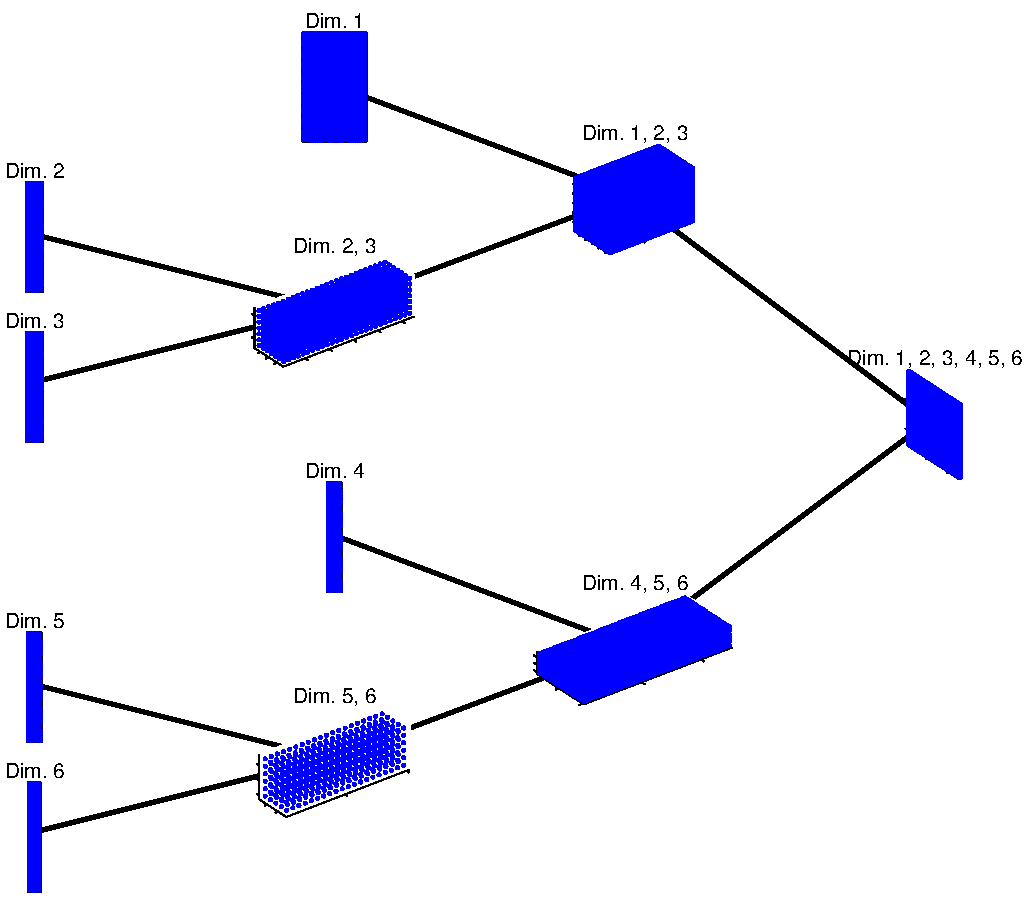
\epsfig{file = spy, scale = 0.35}
      \end{center}
    \end{minipage}$\qquad$
    \begin{minipage}{0.4\textwidth}
      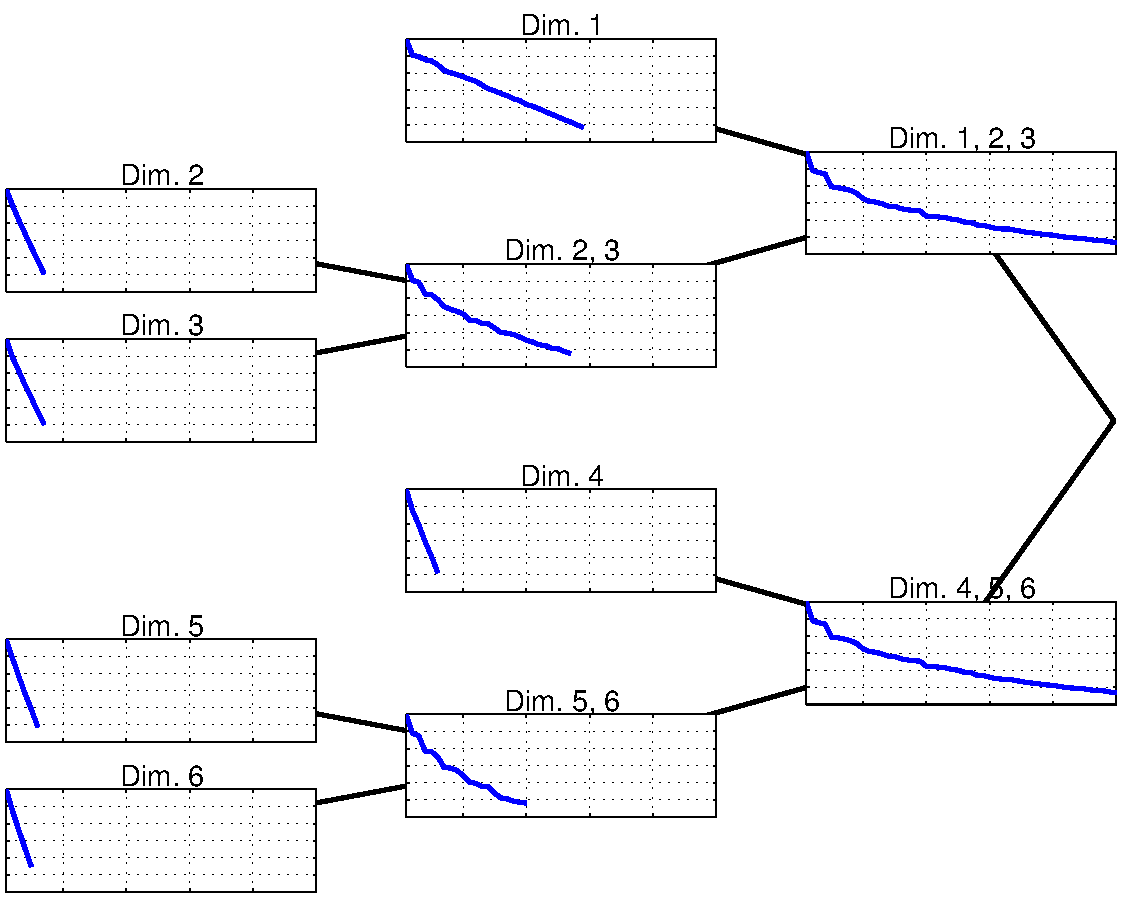
\epsfig{file = plotsv, scale = 0.35}
    \end{minipage}
  \end{center}
  \caption{Examples for \texttt{spy} and \texttt{plot\_sv}} \label{fig:spyplots}
\end{figure}
\end{preprint}

\section{Basic operations} \label{sec:basicops}

This section describes algorithms and implementations for a range of typically required basic operations.

\subsection{$\mu$-mode matrix products}

Given a tensor $\calX \in \C^{n_1\times \cdots \times n_d}$, the $\mu$-mode product
with a matrix $A \in \C^{m\times n_\mu}$ is defined via the $\mu$-mode matricization:
\[
 \calY = A \circ_{\mu} \calX \quad \Leftrightarrow \quad Y^{(\mu)} = A X^{(\mu)}.
\]
This operation can easily be performed if $\calX$ is in HTD: The $\mu$th basis matrix
$U_\mu$ is simply replaced by $A\,U_\mu$. We provide a function {\tt ttm} for performing
this operation. The calling sequence of {\tt ttm} is nearly identical with the function {\tt ttm} in the Tensor Toolbox. A notable difference is that we allow the matrix
the matrix $A$ to be provided implicitly as a 
handle to a function that returns the product of $A$ with the input matrix.
\begin{submitted}
For example, \texttt{y = ttm(x, @(x)(fft(x)), 2)} 
applies the fast Fourier transformation to $\calX$ in mode $2$.
\end{submitted}
\begin{preprint}
\begin{framed}
\noindent \texttt{y = ttm(x, A, 2)} applies the matrix $A$ to an \texttt{htensor} in mode $2$.\\
\texttt{y = ttm(x, \{A, B, C\}, [2, 3, 4])} successively applies $A, B, C$ to $\calX$ in modes $2, 3, 4$.\\
\texttt{y = ttm(x, @(x)(fft(x)), 2)} applies the fast Fourier transformation to $\calX$ in mode $2$.\\
\texttt{y = ttm(x, \{A, B, C\}, [2, 3, 4], 'h')} successively applies $A^H$, $B^H$, $C^H$ to $\calX$ in modes $2, 3, 4$.
\end{framed}
\end{preprint}

\begin{preprint}
In the special case of $\mu$-mode multiplication with a row vector, the $\mu$th mode becomes a
singleton dimension. The function \texttt{ttv} treats this case differently by eliminating
the $\mu$th mode after performing the product $v^T \circ_\mu \calX$
for a vector $v \in \C^{n_\mu}$.
%The only difference is that a singleton dimension is
%created. The function \texttt{ttv} eliminates this singleton
%dimensions, causing the dimension number to change for all dimensions
%greater than $\mu$. The following example illustrates how a dimension
%is eliminated in HTD: we have $u_1^T \in \F^{1 \times k_1}, U_2 \in
%\F^{n_2 \times k_2}$:
%\[
%U_{12} = (U_2 \otimes u_1^T) B_{12} \in \F^{n_2 \times k_{12}}.
%\]
%The nodes $1$ and $2$ are eliminated, and node $(1,2)$ becomes a leaf
%node with matrix $U_{12}$. It remains only to adjust what dimensions
%each node refers to.
The following example illustrates the difference.
\begin{framed}
\noindent \texttt{x = htenrandn([5, 4, 6, 3]); u = randn(4, 1)}; \\
\texttt{y = ttm(x, u.', 2)} results in an \texttt{htensor} $\calY$ of size $5\times 1\times 6\times 3$\\
\texttt{y = ttv(x, u, 2)} results in an \texttt{htensor} $\calY$ of size $5\times 6\times 3$
\end{framed}
\noindent Note that there is also a function \texttt{squeeze} for eliminating
singleton dimensions.
\end{preprint}

\subsection{Addition} \label{sec:explicitaddition}

The addition of tensors in HTD can be performed at no arithmetic cost by a simple embedding. The underlying principle
can easily be seen for two factorized matrices $A = U_A \Sigma_A V_A^H$ and $B = U_B \Sigma_B V_B^H$:  \[
 A+B = \left[\begin{array}{cc}
U_A & U_B
\end{array}
\right]\left[\begin{array}{cc}
\Sigma_A & 0 \\
0 & \Sigma_B
\end{array}
\right]\left[\begin{array}{cc}
V_A & V_B
\end{array}
\right]^H.
\]
This embedding is performed similarly for the addition of two or more tensors in HTD, by
concatenation of the leaf matrices and a block diagonal embedding of the transfer tensors.
We refrain from giving a technical description and refer to Figure~\ref{fig:addition} for an illustration.
\begin{figure}
  \begin{center}
    \resizebox{8cm}{!}{\input addition.eps_t}
  \end{center}
\caption{Addition of four tensors $\calX_1 + \calX_2 + \calX_3 + \calX_4$ in HTD.} \label{fig:addition}
 \end{figure}
It is important to note that the storage requirements grow cubically in the number of tensors to be added
if the block diagonal structure of the transfer tensors is not exploited. Such an alternative method is discussed in Section~\ref{sec:addtruncate}.

\begin{preprint}
Addition is implemented in the command {\tt plus}, which overloads the binary operator {\tt +} for {\tt htucker} objects.
Subtraction is implemented in the command {\tt minus}, which overloads the binary operator {\tt -}.
\end{preprint}

\subsection{Orthogonalization} \label{sec:orthogonalization}

%Starting from the basis matrices $U_t$ in the leaf nodes of a tensor $\calX$ in HTD, we %can recursively
%define $U_t = (U_{t_r} \otimes U_{t_l}) B_t$ for every node $t \in \calT$.
%In the special case when $t$ is a root node, 
%$U_t$ becomes the vectorization of $\calX$.

An HTD of a tensor $\calX$ is called \emph{orthogonalized} if the columns of $U_t$
form an orthonormal basis for each node $t$ except for the root node.
Recall that the basis matrices $U_t$ are defined recursively according to~\eqref{eq:nestedmatrix}.
As will be seen later, orthogonalized HTDs simplify some important operations related to tensor contraction. Moreover, they reduce the risk of numerical cancellation.

We illustrate the process of orthogonalization for the tensor in standard
HTD from Example~\ref{example:d4}:
\[\text{vec}(\calX) = 
(U_4\otimes U_3  \otimes U_2\otimes U_1) (B_{34}\otimes B_{12})  B_{1234}.\]
In the first step, QR decompositions of the basis matrices are performed:
$U_t = \widetilde U_t R_t$ for $t = 1,\ldots,4$. Here and in the following, ``economic'' QR
decompositions~\cite{GolV96} are performed, i.e., $U_t$ and $\widetilde U_t$ have the same
number of columns. Propagating the factors $R_t$ into the transfer matrices
results in
\[
\text{vec}(\calX) = 
(\widetilde U_4\otimes \widetilde U_3 \otimes \widetilde U_2\otimes \widetilde U_1) (\widehat B_{34} \otimes \widehat B_{12})  B_{1234}
\]
with $\widehat B_{34} := (R_4\otimes R_3) B_{34}$, $\widehat B_{12} := (R_2\otimes R_1) B_{12}$. In the next step,
QR decompositions $\widehat B_{34} = \widetilde B_{34} R_{34}$,
$\widehat B_{12} = \widetilde B_{12} R_{12}$ are performed, resulting in 
\begin{equation} \label{eq:orthhtd}
\text{vec}(\calX) = 
(\widetilde U_4\otimes \widetilde U_3  \otimes \widetilde U_2\otimes \widetilde U_1) (\widetilde B_{34} \otimes \widetilde B_{12}) \widetilde B_{1234}
\end{equation}
with $\widetilde B_{1234} := (R_{34}\otimes R_{12}) B_{1234}$.  Clearly,~(\ref{eq:orthhtd}) constitutes
an orthogonalized HTD, completing the orthogonalization procedure.

This procedure easily extends to the general case, see
\begin{preprint}
Algorithm~\ref{alg:orthog}. 
\end{preprint}
\begin{submitted}
 \cite[Alg. 1]{KreT11tr}.
\end{submitted}
Properly implemented, orthogonalization requires $\calO(dnr^2 + dr^4)$ operations. Unless $r$ is very small,
the factor $dr^4$, caused by the QR decompositions of the transfer matrices,
will be dominant.
\begin{preprint}
 \begin{algorithm}
\caption{Orthogonalization of a tensor in HTD}
\label{alg:orthog}
\begin{algorithmic}\small
\REQUIRE Basis matrices $U_t$ and transfer tensors $\calB_t$ defining a general HTD of a tensor $\calX$.
\ENSURE Basis matrices $\widetilde U_t$ and transfer tensors $\widetilde \calB_t$ defining an orthogonalized HTD of $\calX$.
\STATE {\bf for} $t \in \calL(\calT)$: Compute QR decomposition $U_t =: \widetilde U_t R_t$.
\FOR{$t \in \calN(\calT)$ (visiting both child nodes before the parent node)}
  \STATE Form $\widehat B_t = (R_{t_r} \otimes R_{t_l}) B_t$.
\IF{$t$ is root node}
 
\STATE Set $\widetilde B_t = \widehat B_t$.
\ELSE
\STATE Compute QR decomposition $\widehat B_t =: \widetilde B_t R_t$.
\ENDIF
\ENDFOR
\end{algorithmic}
\end{algorithm}
\end{preprint}

In the {\tt htucker} toolbox, orthogonalization is performed by
calling {\tt x = orthog(x)}.
On return, the flag \texttt{is\_orthog} of the {\tt htensor} object {\tt x}
is set to true. This prevents unnecessary orthogonalization in subsequent
calls to {\tt orthog}.
When this property is destroyed by an operation, such as addition and $\mu$-mode matrix 
products, the flag \texttt{is\_orthog} is set to false.
%Therefore repeated orthogonalization is required, which often constitutes the computationally most expensive part of an algorithm.
%In all operations that may destroy orthogonality 
%(e.g., addition of two tensors), the flag \texttt{is\_orthog} is set to false.

\section{Tensor-Tensor Contraction} \label{sec:contraction}

The contraction of two tensors $\calX \in \C^{m_1 \times \cdots \times m_c}$ and $\calY \in
\C^{n_1 \times \cdots \times n_d}$ is a fundamental operation which generalizes the concepts
of inner product, outer product, and matrix multiplication.
In its most general form, we select a tuple of modes $s = (i_1, \ldots, i_p)$ from $\calX$
and another tuple of modes $t = (j_1, \ldots, j_p)$ from $\calY$.
Then the corresponding contraction of 
$\calX$ and $\calY$ amounts to taking the inner product with respect to each
pair $(i_\mu,j_\mu)$ of selected modes. This implicitly assumes that the sizes of the selected modes match, i.e.,
$n_{i_\mu} = m_{j_\mu}$ for $\mu = 1, \ldots, p$. Contraction results in
a tensor $\calZ$ whose order equals the number of non-selected modes.
For example, for $c = 4, d = 3$, and $s = (3,1), t = (2,3)$,
the contracted tensor $\calZ \in \C^{m_2 \times m_4 \times n_1}$
is given by
\begin{equation} \label{eq:contractionxy}
 \calZ_{i_1,i_2,i_3} = 
\innerprod{\calX}{\calY}_{(3, 1),(2, 3)} := \sum_{j=1}^{n_3}
\sum_{k=1}^{n_1} \bar{\calX}_{k,i_1,j,i_2} \calY_{i_3,j,k}.
\end{equation}
A matrix-matrix multiplication $X^H Y$ for $X \in \C^{n_1 \times
  n_2}$, $Y \in \C^{m_1 \times m_2}$ with $n_1 = m_1$ can be seen as
the contraction corresponding to $s = (1)$, $t = (1)$. Conversely, a
general tensor-tensor contraction of $\calX \in \C^{m_1 \times \cdots
  \times m_c}$ and $\calY \in \C^{n_1 \times \cdots \times n_d}$ along
$p$ selected pairs of nodes can be defined via matrix-matrix
multiplication:
\begin{equation} \label{eq:defcontraction}
Z^{(\bar{t})} =  \Big( \innerprod{\calX}{\calY}_{(t; s)} \Big)^{(\bar{t})} :=
(X^{(t)})^H Y^{(s)}, \quad \text{with} \quad \bar{t} = (1, 2, \ldots, c - p).
\end{equation}
Note that the matricization needs to respect the order of the modes in $t$ and $s$, see also Section~\ref{sec:hosvd}.

\subsection{Tensor Network Diagrams}

In the following, we briefly introduce tensor network diagrams (also called
Penrose diagrams)
to conveniently describe algorithms for contractions of tensors in HTD,
see also~\cite{HolRS10b,Huckle2013}. Such a diagram represents a tensor
in terms of contractions of other tensors. Each node in the diagram
represents a tensor and each edge 
represents a mode. An edge connecting two nodes corresponds to the contraction of these tensors
in the associated pair of modes. We allow for dangling edges, which are connected to
only one node and correspond to modes that are not contracted.
Hence, the order of the tensor represented by the network is given by the number of 
dangling edges.

To illustrate the concept of tensor network diagrams, let us consider the contraction given
in~\eqref{eq:contractionxy}. This is represented by the following diagram:
\begin{center}
\resizebox{!}{2cm}{\input{tensor_network_small.pdf_t}}
\end{center}
The node $\calX$ has four edges, each corresponding to one of the four different modes 
of the tensor $\calX$. Similarly, the node $\calY$ has three edges. Since mode $3$
of $\calX$ is contracted with mode $2$ of $\calY$, the nodes share the corresponding edge.
Similarly, the contraction of modes $1$ and $3$ is represented by another shared edge.

Some further examples of tensor network diagrams are given in 
Figure~\ref{fig:tnexamples}. Note that we will only indicate
the precise mode(s) belonging
to an edge when necessary.
\begin{figure}
\begin{center}
  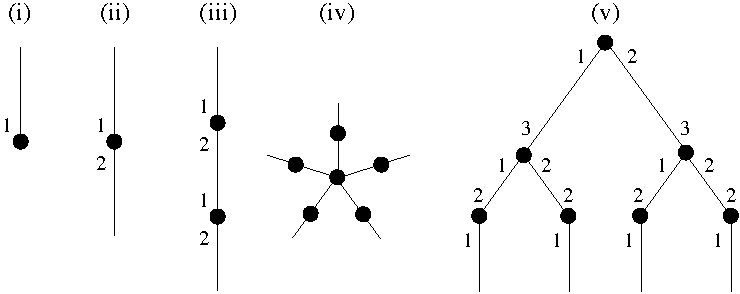
\includegraphics[width=10cm]{tensor_network}
\end{center}
 \caption{Tensor network diagrams representing
(i) a vector, (ii) a matrix, (iii) a matrix-matrix multiplication, (iv) a tensor in Tucker decomposition,
and (v) a tensor in HTD. } \label{fig:tnexamples}
\end{figure}
In the case of HTD, each edge connecting two nodes
corresponds to a matricization $X^{(t)}$ for some $t \in \calT$.

\subsection{Inner Product and Norm for Tensors in HTD} \label{sec:innerprod}

The inner product of two tensors $\calX, \calY \in \C^{n_1 \times \cdots \times n_d}$
is an important special case of
contraction:
\[
\innerprod{\calX}{\calY} = \sum_{i_1=1}^{n_1} \cdots
\sum_{i_d=1}^{n_d} \bar{\calX}_{i_1,\ldots,i_d}
\calY_{i_1,\ldots,i_d}
\] 
or, equivalently, $\innerprod{\calX}{\calY} =
\innerprod{\vect(\calX)}{\vect(\calY)}$. In terms of tensor network diagrams, this operation
corresponds to a pairwise connection of the dangling edges of $\bar{\calX}$ and
$\calY$.

To illustrate how to evaluate inner products of tensors in HTD
efficiently, we first consider two tensors of order $4$:
\[
\innerprod{\calX}{\calY} = (B^x_{1234})^H (B^x_{34} \otimes
B^x_{12})^H (U^x_4 \otimes U^x_3 \otimes U^x_2 \otimes U^x_1)^H (U^y_4
\otimes U^y_3 \otimes U^y_2 \otimes U^y_1) (B^y_{34} \otimes B^y_{12})
B^y_{1234}.
\]
This product is evaluated from inside to outside or, when considering the hierarchical tree, from
the leaves to the root node. In a first step, the matrices
\[
 M_t = \big( U^x_t \big)^H U^y_t, \quad t  = 1,\ldots,4,
\]
are computed. Then the product
\begin{equation} \label{eq:diamondmultiplication}
M_t = (U^x_t)^H U^y_t = (B^x_t)^H \Big(M_{t_r} \otimes
M_{t_l} \Big) B^y_t
\end{equation}
is computed for $t = \{1,2\}$ and $t = \{3,4\}$.
Note that the matrix $M_{t_r} \otimes M_{t_l}$
is not formed explicitly but the matrices
$M_{t_l}$ and $M_{t_r}$ are applied to the modes $1$ and $2$
of $B_t^y$, respectively.
The product~(\ref{eq:diamondmultiplication}) then requires $6r^4$ operations if both
$\calX$ and $\calY$ have constant hierarchical rank $r$.
In the last step, $\innerprod{\calX}{\calY}$ is obtained by evaluating~(\ref{eq:diamondmultiplication})
for $t = \{1,2,3,4\}$.
\begin{figure}
\begin{center}
\begin{tabular}{ccccc}
{\bf Step 1} && {\bf Step 2} && {\bf Step 3} \\[0.3cm]
\resizebox{!}{5.5cm}{\input{innerprod1.pdf_t}} & $\ $ &
\resizebox{!}{5.5cm}{\input{innerprod2.pdf_t}} &$\ $ &
\resizebox{!}{5.6cm}{\input{innerprod3.pdf_t}}
\end{tabular}
  \end{center}
  \caption{Inner product of two tensors of order $4$ in HTD.}
  \label{fig:innerprod}
\end{figure}
Figure~\ref{fig:innerprod} illustrates the described procedure with tensor network diagrams.

The generalization to tensors of arbitrary order is straightforward%
\begin{preprint}
 and summarized in Algorithm~\ref{alg:innerprod}. 
 Note that the
algorithm assumes that $\calX$ and $\calY$ have the same dimension
tree. This requirement can be slightly relaxed as discussed in the
next section for a more general setting.  
\end{preprint}
\begin{submitted}
, see~\cite[Alg. 2]{KreT11tr}, and implemented in
the \htucker{}
function {\tt innerprod}.
\end{submitted}
In total, forming the inner
product of two tensors with constant hierarchical rank $r$ requires
$6(d-1)r^4 + \sum_{\mu = 1}^d 2 n_{\mu} r^2$ operations.
\begin{preprint}
Algorithm~\ref{alg:innerprod} is implemented in the \htucker{}
function {\tt innerprod}.
\begin{algorithm}
  \caption{Inner product of two tensors in HTD}
  \label{alg:innerprod}
  \begin{algorithmic}\small
    \REQUIRE Tensors $\calX, \calY$ in HTD, of equal dimension tree $\calT$
    and equal size $n_1 \times \cdots \times n_d$, defined by basis
    matrices $U^x_t, U^y_t$ and transfer tensors $\calB^x_t,
    \calB^y_t$.
    % , matrices $U^x_t, U^y_t$ for all leaf nodes $t \in
    % \calL(\calT)$, third order tensors $\calB^x_t, \calB^y_t$ for
    % all non-leaf nodes $t \in \calN(\calT)\setminus\{r\}$, and
    % $\calB^x_r, \calB^y_r$.
    \ENSURE Inner product $\innerprod{\calX}{\calY}$.
    \FOR{$t \in \calL(\calT)$}
    \STATE Form $M_t = (U^x_t)^H U^y_t$.
    \ENDFOR
    \FOR{$t \in \calN(\calT)$ (visiting both child nodes before the parent node)} 
    \STATE Form $M_t = (B^x_t)^H \big( M_{t_r} \otimes M_{t_l} \big) (B^y_t)$.
    \ENDFOR
    \STATE Return $\innerprod{\calX}{\calY} = M_{t_\text{root}}$.
  \end{algorithmic}
\end{algorithm}
\end{preprint}

In principle, the Euclidean norm of a tensor $\calX$ in HTD
can be calculated from $\| \calX \|_2 = \sqrt{\innerprod{\calX}{\calX}}$ by
means of an inner product. However, it is well
known that such an approach suffers from numerical instabilities and
may introduce an error proportional to the square root of machine precision.
A usually more accurate alternative is to first orthogonalize the HTD of $\calX$
and then compute the norm.
\begin{preprint}
 Note that the second part is trivial; it is
easy to see that $\|\calX\|_2 = \|\calB_{1,2,\ldots,d}\|_F$ in the case of an orthogonalized
HTD. The orthogonalization step makes the second approach slightly more expensive.
The accuracy difference between the two approaches is 
illustrated in the following \textsc{Matlab} example.
%
\begin{framed}\noindent
\vspace{-2ex}
\begin{verbatim}
x = htenrandn([5, 4, 6, 3]);
norm(x - x)/norm(x)
1.5355e-08
norm(orthog(x - x))/norm(x)
5.6998e-16
\end{verbatim}
\vspace{-2ex}
\end{framed}
\end{preprint}

\subsection{General Contraction of Tensors in HTD} \label{sec:generalcontraction}

In tensor network diagrams, a general contraction of two tensors in HTD 
is performed by connecting the corresponding pairs of dangling edges. This
will create a tensor network with cycles, which need to be eliminated.
This elimination is performed by successive contraction of tensors, similarly
as above, until the network becomes a tree.
\begin{submitted}
 Note that this procedure can only be organized efficiently if 
the maximum degree of all intermediate tensor networks does not become too large.
In turn, this imposes certain restrictions on the input data to the function {\tt ttt}
that implements a general contraction. For details, we refer to~\cite[Sec. 3.5.2]{Tob12}.
\end{submitted}
\begin{preprint}
 This can only be organized efficiently if 
the maximum degree of all intermediate tensor networks does not become too large.
Figure~\ref{fig:excessivedegree} provides a simple example where the maximum degree
inevitably grows.
\begin{figure}
\begin{center}
\resizebox{9cm}{!}{\input{triangle1.pdf_t}}
  \end{center}
  \caption{Example for which the elimination of a cycle creates a temporary node of larger degree.}
  \label{fig:excessivedegree}
\end{figure}
To avoid this effect, we \emph{assume} that the maximum degree remains at most $3$.
This also ensures that the eventually obtained tensor network 
corresponds to an HTD. In fact, the super node 
containing the aggregation of all cycles can be shown to have degree $2$. Hence, it is natural
to use this node as the root node in the HTD of the contraction.

Under the conditions mentioned above, the algorithm for performing a general contraction is a direct, but rather technical extension
of Algorithm~\ref{alg:innerprod}. For implementation details, we refer to~\cite[Sec. 3.5.2]{Tob12} and the source code of the function \texttt{ttt}
in the \texttt{htucker} toolbox, which provides an implementation of the sketched algorithm.
\begin{framed} \noindent
\noindent
  \texttt{x = htenrandn([4, 2, 3]);} \texttt{y = htenrandn([3, 4, 2]);} \\
  \texttt{z = ttt(x, y,[1 3],[2 1]);} Contracted product, connecting
  mode $1$ of $\calX$ with mode $2$ of $\calY$, and
  mode $2$ of $\calX$ with mode $1$ of $\calY$. Results in $\calZ \in \R^{2 \times 2}$. \\
  \texttt{ttt(x, x, 1:3);} Inner product, identical with \texttt{innerprod(x, x)}.\\
  \texttt{z = ttt(x, y);} Outer product $\calZ \in \R^{4 \times 2 \times 3 \times 3 \times 4 \times 2}$.
\end{framed}
\end{preprint}

\subsection{Reduced Gramians of a Tensor in HTD} \label{sec:reducedgramians}

An important application of contractions is the calculation of reduced Gramians, which
are defined as follows.
For every $t \in \calT$, the matrix $U_t$ defined in~(\ref{eq:nestedmatrix})
contains a basis for the column span of the matricization $X^{(t)}$. Hence,
there is a matrix $V_t$ such that $X^{(t)} = U_t V_t^H$. 
The \emph{reduced Gramian} at $t$ is then defined as the
Hermitian positive semi-definite matrix $G_t = V_t^H V_t \in \C^{r_t\times r_t}$.

Reduced Gramians are a central tool in the truncation
of tensors. For example, they provide an efficient way to compute
the singular values of $X^{(t)}$, which is used in the function {\tt plot\_sv}.
From
\begin{equation} \label{eq:matrixgramian}
 X^{(t)} (X^{(t)})^H = U_t V_t^H V_t U_t^H = U_t G_t U_t^H
\end{equation}
it follows that the singular values of $X^{(t)}$ are the square roots of the eigenvalues 
of the reduced Gramian $G_t$, provided that $U_t^H U_t = I_{r_t}$. This condition is always satisfied after
the HTD has been orthogonalized.

In the following, we briefly discuss the computation of a reduced Gramian $G_t$ via contraction. The
standard, unreduced Gramian corresponds to the contracted product of $\calX$ with itself along
the modes $t^c = \{1,\ldots,d\}\setminus t$: $\overline{\innerprod{\calX}{\calX}_{t^c}}$,
for which the matricization is given by~(\ref{eq:matrixgramian}), see also Figure~\ref{fig:gramian_8} for an illustration.
It can be seen from the figure
%, and it is true in general, that
%$G_t$ happens to be the super node $\calC$ from Section~\ref{sec:generalcontraction}, containing the aggregation of all cycles.%
\begin{figure}
  \begin{center}
    \resizebox{5cm}{!}{\input{gramian_8.eps_t}}
  \end{center}
  \caption{Reduced Gramian of a tensor of order $8$. The reduced
    Gramian $G_t$ corresponds to the left subnetwork encircled by a dashed line.}
  \label{fig:gramian_8}
\end{figure}%
%
%
\begin{figure}
  \begin{center}
    \resizebox{12cm}{!}{\input{gramian_recursion.pdf_t}}
  \end{center}
  \caption{How to calculate $G_{t_r}$ from $G_t$, $U_{t_l}$ and $B_t$,
    where $t$ is a general non-leaf node. The gray lines represent
    arbitrary subtrees.}
  \label{fig:gramian_recursion}
\end{figure}
%
that Gramians are closely related to contraction. In particular, this relation implies that $G_t$ can be calculated by a sequence of matrix-tensor and
tensor-tensor products%
\begin{preprint}
, similar to Algorithm~\ref{alg:innerprod}.
\end{preprint}
\begin{submitted}
.
\end{submitted}

Typically, not the reduced Gramian at one node $t$ is required, but
reduced Gramians $G_t$ for all nodes $t \in \calT$. These can be computed
simultaneously by exploiting
relations between different reduced Gramians.
The relationship between the reduced Gramians $G_t$
and $G_{t_r}$, where $t_r$ is the right child node of $t$, is
illustrated in Figure~\ref{fig:gramian_recursion} for the case of a
general non-leaf node $t$. From the tensor network diagram, it can be seen that
\begin{equation} \label{eq:gramian_recursion}
  \begin{aligned}
    G_{t_r} &= (B_t^{(\{1, 3\})})^H (G_t \otimes U_{t_l}^H U_{t_l} ) B_t^{(\{1,3\})}, \\
    % \innerprod{\calB_t}{G_t \circ_3 (U_{t_l}^H U_{t_l}) \circ_1 \calB_t}_{(1, 3)} = 
    G_{t_l} &= (B_t^{(\{2,3\})})^H (G_t \otimes U_{t_r}^H U_{t_r}) B_t^{(\{2,3\})}. \\
    %\innerprod{\calB_t}{G_t \circ_3 (U_{t_r}^H U_{t_r}) \circ_2 \calB_t}_{(2, 3)} = 
  \end{aligned}
\end{equation}
Formally setting $G_{t_\text{root}} = 1$, this defines a recursive
algorithm for the calculation of all reduced Gramians%
\begin{submitted}
.
\end{submitted}
\begin{preprint}
, see
Algorithm~\ref{alg:reducedgramians}.
\end{preprint}
An efficient algorithm
for calculating $M_t = U_t^H U_t$ is already described in Section~\ref{sec:innerprod}%
\begin{preprint}
and given in
Algorithm~\ref{alg:innerprod}. 
\end{preprint}
\begin{submitted}
.
\end{submitted}
Note that all $M_t$
are identity matrices for a tensor in orthogonalized HTD.

For a general HTD,
\begin{preprint}
Algorithm~\ref{alg:reducedgramians}
\end{preprint}
\begin{submitted}
the computation of the reduced Gramians
\end{submitted}
requires $O(dnr^2 + (d-2)r^4)$ operations. For an orthogonalized HTD,
this reduces to $O((d-2)r^4)$ operations (but orthogonalization itself requires $O(dnr^2 + (d-2)r^4)$ operations).

\begin{framed} \noindent
\texttt{G = gramians(x);} Reduced Gramians of $\calX$ in cell array \texttt{G}, orthogonalizing the HTD of $\calX$ if necessary.\\
\texttt{G = gramians\_nonorthog(x);} Reduced Gramians of $\calX$ in cell array \texttt{G}, without orthogonalizing.\\
\texttt{sv = singular\_values(x);} Singular values of $\calX$ in cell array \texttt{sv}.
%\texttt{plot\_sv(x);} Plot tree of singular values at every node.
\end{framed}
%
\begin{preprint}
 \begin{algorithm}
  \caption{Reduced Gramians of a tensor in HTD}
  \label{alg:reducedgramians}
  \begin{algorithmic}\small
    \REQUIRE Basis matrices $U_t$ and transfer tensors $\calB_t$
    defining a general HTD of a tensor $\calX$.
    \ENSURE Reduced Gramians $G_t$ for all $t \in \calT$.
    \FOR{$t \in \calL(\calT)$}
    \STATE Form $M_t = (U_t)^H U_t$.
    \ENDFOR
    \FOR{$t \in \calN(\calT)$ (visiting both child nodes before the parent node)} 
    \STATE Form $M_t = (B_t)^H \big( M_{t_r} \otimes M_{t_l} \big) (B_t)$.
    \ENDFOR
    \STATE Set $G_{t_\text{root}} = 1$.
    \FOR{$t \in \calN(\calT)$ (visiting parent nodes before their children)} 
    \STATE Form $G_{t_r} = (B_t^{(\{1,3\})})^H (G_t \otimes M_{t_l} ) B_t^{(\{1,3\})}$.
    \STATE Form $G_{t_l} = (B_t^{(\{2,3\})})^H (G_t \otimes M_{t_r} ) B_t^{(\{2,3\})}$.
    \ENDFOR
  \end{algorithmic}
\end{algorithm}
\end{preprint}


\section{Truncation of tensors} \label{sec:truncation}

Truncation of tensors to HTD is one of the most important and most frequently used operations in \htucker.

\subsection{Truncation of explicit tensors}

We start with the truncation of an explicitly given tensor $\calX \in
\C^{n_1 \times \cdots \times n_d}$.  Although this situation is
limited to small dimensions/sizes, it provides a gentle introduction
and illustration of the general concepts. Truncation to HTD is done by
successive projections to the subspaces $\text{span}(W_t)$, which
typically represent approximations to the column spaces of $X^{(t)}
\in \C^{n_t \times n_{t^c}}$. For a subset $t \subset \{1, \ldots, d\}$,
we define $n_t := \prod_{\mu \in t} n_\mu$.  We require $W_t \in
\C^{n_t \times r_t}$ to have orthonormal columns and define the
orthogonal projections 
\begin{equation} \label{eq:defproj}
\pi_t := W_t W_t^H.
\end{equation}
In the following, we use the shorthand notation $\pi_t \calX$ for
$\pi_t \circ_t \calX$. As shown in~\cite[Lemma 3.15]{Gra10}, applying
these projections in the correct order leads to a tensor in HTD, with
hierarchical ranks bounded by $r_t$.
%
\subsubsection{Root-to-leaves truncation} \label{sec:RtL}

The simplest way to construct the projections $\pi_t$ in~(\ref{eq:defproj}) is to
let each matrix $W_t$ contain the $r_t$ dominant left singular
vectors of the corresponding matricization $X^{(t)}$. To obtain a tensor in
HTD, $\tilde{\calX} \in
\HTucker\big((r_t)_{t\in\calT}\big)$, the projections need to be applied 
from the root node to the leaves.
\begin{preprint}
This is illustrated by the following example for order $4$:
\begin{align}
  \vect(\tilde \calX) &= (W_4 W_4^H \otimes W_3 W_3^H \otimes W_2 W_2^H
  \otimes W_1 W_1^H)
  (W_{34} W_{34}^H \otimes W_{12} W_{12}^H) \vect(\calX) \label{eq:examplertl} \\
  &= (W_4 \otimes W_3 \otimes W_2 \otimes W_1) ( \underbrace{[W_4^H
    \otimes W_3^H] W_{34}}_{=: B_{34}} \otimes \underbrace{[W_2^H
    \otimes W_1^H] W_{12}}_{=: B_{12}} ) \underbrace{([W_{34}^H
    \otimes W_{12}^H] \vect(\calX))}_{=: B_{1234}}. \nonumber
\end{align}
The computation for the general case is
described in Algorithm~\ref{alg:trunc_RtL}. Note that the HTD of
the resulting tensor is not 
orthogonalized, only the matrices in the leaf nodes have orthonormal columns.
%
\begin{algorithm}
\caption{Root-to-leaves truncation of a tensor}
\label{alg:trunc_RtL}
\begin{algorithmic}\small
  \REQUIRE Tensor $\calX \in \C^{n_1 \times \cdots \times n_d}$,
  dimension tree $\calT$ and desired hierarchical ranks $(r_t)_{t \in
    \calT}$ of the truncated tensor.
  \ENSURE Tensor $\tilde{\calX}$ in HTD, with $\rank (\tilde{X}^{(t)}) \le r_t$ for all $t \in \calT$.
  \FOR{$t \in \calT$ (visiting both child nodes before the parent node)}
  \IF{$t \in \calL(\calT)$}
  \STATE Compute singular value decomposition $X^{(t)} =: \hat{U}_t \hat{\Sigma}_t \hat{V}_t^H$.
  \STATE Set $U_t := \hat{U}_t(:, 1:r_t)$.
  \ELSIF{$t$ is the root node}
  \STATE Form $B_t := (U_{t_r}^H \otimes U_{t_l}^H) \vect(\calX)$.
  \ELSE
  \STATE Compute singular value decomposition $X^{(t)} =: \hat{U}_t \hat{\Sigma}_t \hat{V}_t^H$.
  \STATE Set $U_t := \hat{U}_t(:, 1:r_t)$.
  \STATE Form $B_t := (U_{t_r}^H \otimes U_{t_l}^H) U_t$.
  \ENDIF
  \ENDFOR
  
\end{algorithmic}
\end{algorithm}
\end{preprint}
%
\begin{submitted}
  The computation for the general case is described in
  \cite[Alg. 1]{Gra10} and \cite[Alg. 4]{KreT11tr}. Note that the HTD
  of the resulting tensor is not orthogonalized, only the matrices in
  the leaf nodes have orthonormal columns.
\end{submitted}
% 
Setting $n = \max_t n_t$, the computational complexity
of root-to-leaves truncation is of order $d n^{3d/2}$ in the case of a
balanced tree. 
\begin{preprint}
An efficient way to calculate $W_t$ is
through an eigenvalue decomposition of the Gramian: $X^{(t)} (X^{(t)})^H = W_t \Sigma^2 W_t^H$.
\end{preprint}
The resulting tensor $\tilde{\calX}$ satisfies the following error bound~\cite[Theorem 3.11]{Gra10}:
  \begin{equation} \label{eq:errorboundltr}
  \normb{\calX - \tilde \calX}_2
  \le \sqrt{ \sum_{t \in \calT'} \delta_{r_t}(X^{(t)})^2 } 
  \le \sqrt{2d - 3} \: \normb{ \calX - \calX_{\text{best}} }_2,
  \end{equation}
  where $\calX_{\text{best}}$ represents the best approximation of
  $\calX$ in $\calH$-Tucker$((r_t)_{t \in \calT})$, $\calT' := \calT \setminus \{t_\text{root}, t_\text{child} \}$ where $t_\text{child}$ is a child of the root node $t_\text{root}$, and
\begin{equation} \label{eq:delta}
 \delta_{r_t}(X^{(t)})^2:=\sum_{j=r_t+1}^{n_t} \sigma_j(X^{(t)})^2.
\end{equation}

\begin{remark}
The error bound~(\ref{eq:errorboundltr}) allows us to choose the
hierarchical ranks $(r_t)_{t \in \calT}$ such that a certain
error bound is satisfied:
  \begin{align*}
  \normb{ \calX - \tilde{\calX} }_2
  \le \epsilon_\text{abs}, 
  \quad \text{choose $r_t$ s.t.} \quad
  \delta_{r_t}(X^{(t)})
  \le \frac{\epsilon_\text{abs}}{\sqrt{2d-3}} 
  \quad \forall t \in \calT\setminus\{t_\text{root}\},\\
  \normb{ \calX - \tilde{\calX} }_2 
  \le \epsilon_\text{rel} \: \norm{\calX}_2, 
  \quad \text{choose $r_t$ s.t.} \quad
  \delta_{r_t}(X^{(t)})
  \le \frac{\epsilon_\text{rel} \: \norm{\calX}_2}{\sqrt{2d-3}} 
  \quad \forall t \in \calT \setminus\{t_\text{root}\}.
  \end{align*}
  Similar adaptive choices of the hierarchical ranks are possible for all other truncation methods discussed in the following.
\end{remark}
%
\begin{framed} \noindent
\texttt{opts.max\_rank = 10;} maximal rank at truncation, mandatory argument.\\
\texttt{opts.rel\_eps = 1e-6;} maximal relative truncation error, optional argument.\\
\texttt{opts.abs\_eps = 1e-6;} maximal absolute truncation error, optional argument.\\
Condition \texttt{max\_rank} takes precedence over \texttt{rel\_eps} and \texttt{abs\_eps}.\\
\texttt{y = htensor.truncate\_rtl(x, opts);} takes a \textsc{Matlab} multidimensional array and returns the truncation to lower rank HTD.
\end{framed}

\subsubsection{Leaves-to-root truncation} \label{sec:LtR}

Root-to-leaves truncation is very costly, the most expensive part
being the computation of the singular value decomposition of every $X^{(t)}
\in \C^{n_t \times n_{t^c}}$, where both $n_t$ and $n_{t^c}$ can become very large.
Leaves-to-root truncation can be considerably faster.
\begin{submitted}
It is described in \cite[Alg. 2]{Gra10} and \cite[Alg. 5]{KreT11tr}, and implemented in the function \texttt{x = htensor.truncate\_ltr(x, opts)} of the toolbox.
\end{submitted}
\begin{preprint}
To illustrate the idea, consider a fourth order
tensor. For each leaf node $t$, we define $W_t$ to contain the $r_t$ dominant left 
singular vectors of $X^{(t)}$ and set
\[
\vect(\calC_{1}): = (W_4^H \otimes W_3^H \otimes W_2^H \otimes W_1^H) \vect(\calX), \quad \calC_{1} \in \C^{r_1 \times r_2 \times r_3 \times r_4}.
\]
In the next step, we consider the nodes
$t = \{1,2\}, t = \{3,4\}$, and define
$S_t$ to contain the $r_t$ dominant left singular vectors of $C_{1}^{(t)}$:
\[
\vect(\calC_{0}) = (S_{34}^H \otimes S_{12}^H) \vect(\calC_{1}), \quad \calC_{0} \in \C^{r_{12} \times r_{34}}.
\]
The resulting tensor is in HTD:
\[
\vect(\tilde{\calX}) = (W_4 \otimes W_3 \otimes W_2 \otimes W_1)
(S_{34} \otimes S_{12}) \vect(\calC_{0}).
\]
For the case of a general tensor, see
Algorithm~\ref{alg:trunc_LtR}.
Note that $h(\mathcal T)$ denotes the height of $\calT$, and the set of all nodes 
with distance $\ell$ ($\ell = 0,\ldots,h(\calT)$) to the root node is denoted by $\calT_{\ell}$.

Algorithm~\ref{alg:trunc_LtR} can be interpreted in
terms of projections $W_t W_t^H$, with the definition $W_t = (W_{t_r}
\otimes W_{t_l}) S_t$. As the subspaces defined by $W_t$
are nested, it can be seen that all projections $\pi_t$ commute, see also Lemma~B.1.
Combined with~\cite[Lemma 3.15]{Gra10}, this shows that the resulting tensor is
in $\HTucker((r_t)_{t \in \calT})$.
%
\begin{algorithm}
\caption{Leaves-to-root truncation of a tensor}
\label{alg:trunc_LtR}
\begin{algorithmic}\small
  \REQUIRE Tensor $\calX \in \C^{n_1 \times \cdots \times n_d}$,
  dimension tree $\calT$ and desired hierarchical ranks $(r_t)_{t \in
    \calT}$ of the truncated tensor.
  \ENSURE Tensor $\tilde{\calX}$ in HTD, with $\rank (\tilde{X}^{(t)}) \le r_t$ for all $t \in \calT$.
  
  \FOR{$t \in \calL(\calT)$}
  \STATE Compute singular value decomposition $X^{(t)} =: \hat{U}_t \hat{\Sigma}_t \hat{V}_t^H$.
  \STATE Set $\tilde{U}_t := \hat{U}_t(:, 1:r_t)$.
  \ENDFOR
  \STATE Form $\calC_{L-1} := (\tilde U_d^H \otimes \cdots \otimes \tilde U_1^H) \calX$.
  \FOR{$\ell = h(\calT)-1, \ldots, 1$}
  \FOR{$t \in \calT_\ell \setminus \calL(\calT)$}
  \STATE Compute singular value decomposition  $C_\ell^{(t)} =: \hat{S}_t \hat{\Sigma}_t \hat{V}_t^H$.
  \STATE Set $B_t := \hat{S}_t(:, 1:r_t)$.
  \ENDFOR
  \STATE Form $\calC_{\ell-1} := \Big( \prod_{t \in \calT_\ell} B_t^H \circ_t \Big) \calC_\ell$.
  \ENDFOR
  \STATE Set $B_{t_\text{root}} := \vect(\calC_0)$.
\end{algorithmic}
\end{algorithm}
\end{preprint}
The computational complexity of leaves-to-root truncation
%, when
%using Gramians to calculate the left
%singular vectors,
is $O(d n^{d+1})$, which is a significant reduction
compared to the root-to-leaves method, while the error bound~(\ref{eq:errorboundltr})
still holds, see Lemma B.2%
\begin{preprint}
.
\end{preprint}
\begin{submitted}
{} in~\cite{KreT11tr}.
\end{submitted}
Moreover, the resulting tensor
$\tilde{\calX}$ is in orthogonalized HTD.
% 
\begin{preprint}
\begin{framed} \noindent
\texttt{x = htensor.truncate\_ltr(x, opts);} takes a \textsc{Matlab} multidimensional array and returns the truncation to lower rank HTD.
\end{framed}
\end{preprint}
%
\subsection{Truncation of $\calH$-Tucker decomposition to lower rank} \label{sec:trunc_htucker}
%

The truncation of a tensor which is already given in HTD to a tensor in HTD of lower rank is
an essential operation in most algorithms based on this format.
In Section~\ref{sec:trunc_std}, we
describe an efficient method for performing such a truncation.
This will be the method of choice for general tensors. However, for structured 
tensors resulting, e.g., from the addition of several tensors in HTD,
a different approach described  in Section~\ref{sec:trunc_var} is preferable.
 
%
\subsubsection{Truncation of a tensor in HTD} \label{sec:trunc_std}
% 
Truncation of a tensor $\calX$ in HTD can be performed by a fairly straightforward adaptation 
of the root-to-leaves method. For this purpose, we recall that Section~\ref{sec:reducedgramians}
describes an efficient method for computing the reduced Gramians $G_t$ in the decomposition
\[
X^{(t)} (X^{(t)})^H = U_t G_t U_t^H,
\]   
where $U_t$ has orthonormal columns and is implicitly represented as illustrated in Figure~\ref{fig:gramian_recursion}.
After orthogonalizing the HTD of $\calX \in \HTucker\big((k_t)_{t\in\calT}\big)$ and calculating the reduced Gramians, we compute
an orthonormal basis $S_t \in \C^{k_t\times r_t}$ for the $r_t$ dominant eigenvectors of the symmetric matrix $G_t$.
As above, we define $W_t := U_t S_t$ and obtain the truncated tensor $\tilde \calX$ from subsequent application
of the projections $\pi_t = W_t W_t^H$.

To illustrate how these projections can be applied to a tensor in HTD, let us consider 
the example of a tensor $\calX$ of order $4$:
\begin{align*}
  \vect(\tilde \calX) &= (W_4 W_4^H \otimes W_3 W_3^H \otimes W_2 W_2^H
  \otimes W_1 W_1^H) (W_{34} W_{34}^H \otimes W_{12} W_{12}^H) \vect(\calX)\\
  %&(U_4 \otimes U_3 \otimes U_2 \otimes U_1) (B_{34} \otimes B_{12}) B_{1234}\\
  &=(U_4 S_4 \otimes U_3 S_3 \otimes U_2 S_2 \otimes U_1 S_1) \cdots \\
& \ \ \ \ \cdots
  (\underbrace{(S_4^H \otimes S_3^H) B_{34} S_{34}}_{=:\tilde{B}_{34}} \otimes \underbrace{(S_2^H \otimes S_1^H) B_{12} S_{12}}_{=:\tilde{B}_{12}}) 
  \underbrace{(S_{34}^H \otimes S_{12}^H) B_{1234}}_{=:\tilde{B}_{1234}}.
\end{align*}
Hence, an HTD for $\tilde \calX$ is obtained by updating the leaf matrices $\tilde U_1 := U_1 S_1$, $\ldots$, 
$\tilde U_4 := U_4 S_4$, and the transfer matrices. Note that the matrices $W_t$ are never calculated explicitly.

\begin{preprint}
This update can be extended to the general case in a direct way:
\[ \begin{array}{rcll}
  \tilde{U}_t &:=& U_t S_t \qquad & \forall t \in \calL(\calT), \\
  \tilde{B}_t &:=& (S_{t_r}^H \otimes S_{t_l}^H) B_t S_t & \forall t \in \calN(\calT).
   \end{array}
\]
Note that the update for the root node $t\equiv t_{\text{root}}$ simplifies to $\tilde{B}_t := (S_{t_r}^H \otimes S_{t_l}^H) B_t$.

%
\begin{algorithm}
  \caption{Truncation of a tensor in HTD}
  \label{alg:trunc_htucker}
  \begin{algorithmic}\small
    \REQUIRE Tensor $\calX$ in HTD and desired hierarchical ranks $(r_t)_{t \in \calT}$ of the truncated tensor.
    \ENSURE Tensor $\tilde{\calX}$ in HTD, with $\rank(\tilde{X}^{(t)}) \le r_t \quad \forall t \in \calT$.
    \STATE Orthogonalize $\calX$ (as described in Algorithm~\ref{alg:orthog}).
    \STATE Calculate reduced Gramians $G_t$ (as described in Algorithm~\ref{alg:reducedgramians}).
    \FOR{$t \in \calT \setminus \{t_{\text{root}}\}$}
    \STATE Compute symmetric eigenvalue decomposition $G_t =: \hat{S}_t \hat{\Sigma}_t^2 \hat{S}_t^H$.
    \STATE Set $S_t := \hat{S}_t(:, 1:r_t)$.
    \ENDFOR
    \STATE $S_{t_{\text{root}}} = 1$
    \STATE {\bf for} $t\in \calL(\calT)$: Set $\tilde{U}_t := U_t S_t$. 
    \STATE {\bf for} $t\in \calN(\calT)$: Set $\tilde{B}_t := (S_{t_r}^H \otimes S_{t_l}^H) B_t S_t$.
  \end{algorithmic}
\end{algorithm}
\end{preprint}
%
\begin{preprint}
Algorithm~\ref{alg:trunc_htucker},
\end{preprint}
\begin{submitted}
Algorithm~6 in \cite{KreT11tr},
\end{submitted}
which describes this procedure, is implemented in \texttt{truncate\_std(x, opts)}, and requires $O(dnr^2 + dr^4)$ operations.
 As this algorithm is mathematically identical to the explicit root-to-leaves algorithm described in Section~\ref{sec:RtL},
the error bound~(\ref{eq:errorboundltr}) holds. Note that the resulting tensor
$\tilde{\calX}$ is not in orthogonalized HTD.
%
\begin{preprint}
\begin{framed} \noindent
\texttt{xt = truncate\_std(x, opts);} takes an {\tt htensor} $\calX$ and returns a truncated {\tt htensor}
$\tilde \calX$.
\end{framed}
\end{preprint}
%
\subsubsection{Truncation of a tensor in HTD without initial orthogonalization} \label{sec:trunc_var}
%

The method of truncation introduced in the last section represents the
default method for truncating a tensor in HTD.  However, in certain
situations, it can be beneficial to exploit additional structure in
the HTD. For example, a tensor resulting from addition of tensors in
HTD has block diagonal transfer tensors. In the standard method of
truncation, such structures are immediately destroyed by the initial
orthogonalization step. In the following, we discuss a method that
avoids this step.
%The resulting method is quite similar to the leaves-to-root
%method.
%Note that, without exploiting such a structure, this second
%method is slightly more expensive than the standard method.

In a first step, the reduced Gramians $G_t$ in the decomposition
\[
X^{(t)} (X^{(t)})^H = U_t G_t U_t^H
\]
are calculated without the initial orthogonalization.
Note, however, that the singular value decomposition of $X^{(t)}$ 
cannot be computed directly from $G_t$,
as the columns of $U_t$ are not orthonormal.

In a second step,
the proposed method successively orthonormalizes the matrices $U_t$.
Let us first consider the leaf nodes $t$, for which
we compute the $r_t$ dominant left 
singular vectors of $X^{(t)}$ as follows: 
Compute the QR decomposition $U_t =: Q_t R_t$, 
and
determine the matrix $S_t$ containing the
$r_t$ dominant eigenvectors of $R_t G_t R_t^H$.
Then the projection $\pi_t = W_t W_t^H$, 
with $W_t = Q_t S_t$, 
is applied to $\calX$.
Note that the updated leaf nodes $\tilde{U}_t:=Q_t S_t$
are orthonormal.

Non-leaf nodes are processed in a similar manner with 
a recursive algorithm,
traversing the tree
such that every parent node is visited
after its child nodes.
Assume we are at node $t$, and let 
$\tilde{U}_t$ account for all updates from previous operations on the descendants of $t$.
Based on the original decomposition $X^{(t)} = U_t V_t^H$, we set
$\tilde{X}_t^{(t)} := 
\tilde{U}_t V_t^H$ and observe that the corresponding Gramian takes the form
\[
\tilde{X}_t^{(t)} (\tilde{X}_t^{(t)})^H = 
\tilde{U}_t G_t \tilde{U}_t^H.
\]
To orthogonalize $\tilde{U}_t = (\tilde{U}_{t_r} \otimes \tilde{U}_{t_l}) \tilde{B}_t$,
it is sufficient to calculate the QR decomposition of
$\tilde{B}_t = (S_{t_r}^H R_{t_r} \otimes S_{t_l}^H R_{t_l}) B_t$, as the columns of $\tilde{U}_{t_l}$ and $\tilde{U}_{t_r}$ are
orthonormal. Then, we calculate the $r_t$ dominant left singular vectors
of $\tilde{X}_t^{(t)}$ as in the case of the leaf nodes.

A more detailed description of truncation to HTD without initial orthogonalization
can be found in 
\begin{preprint}
Algorithm~\ref{alg:trunc_htucker_2}.
\end{preprint}
\begin{submitted}
Algorithm~7 in \cite{KreT11tr}, and is implemented in \texttt{truncate\_nonorthog(x, opts)} in the toolbox.
\end{submitted}
The result of this algorithm satisfies practically the same error bound as 
in~(\ref{eq:errorboundltr}), see also Lemma B.3%
\begin{preprint}
.
\end{preprint}
\begin{submitted}
{} in~\cite{KreT11tr}.
\end{submitted}

\begin{preprint}
The computational complexities of Algorithm~\ref{alg:trunc_htucker} and Algorithm~\ref{alg:trunc_htucker_2}
are the same, but the latter requires more operations.
%
\begin{algorithm}
  \caption{Truncation of a tensor in HTD without initial orthogonalization}
  \label{alg:trunc_htucker_2}
  \begin{algorithmic}\small
    \REQUIRE Tensor $\calX$ in HTD and desired hierarchical ranks $(r_t)_{t \in \calT}$ of the truncated tensor.
    % : tree $\calT$, matrices $U_t$ for all leaf nodes $t \in
    % \calL(\calT)$, third order tensors $\calB_t$ for all non-leaf
    % nodes $t \in \calN(\calT)\setminus\{r\}$, and $\calB_r$,
    \ENSURE Tensor $\tilde{\calX}$ in HTD, with $\rank(\tilde{X}^{(t)}) \le r_t$.
    \STATE Calculate reduced Gramians $G_t$ (as described in Algorithm~\ref{alg:reducedgramians}).
    \FOR{$t \in \calL(\calT)$}
    \STATE Compute QR decomposition $U_t =: Q_t R_t$.
    \STATE Compute symmetric eigenvalue decomposition $R_t G_t R_t^H =: \hat{S}_t \hat{\Sigma}_t^2 \hat{S}_t^H$.
    \STATE Set $S_t := \hat{S}_t(:, 1:r_t)$.
    \STATE Form $U_t := Q_t S_t$.
    \ENDFOR
    \FOR{$t \in \calN(\calT)\setminus\{t_\text{root}\}$ (visiting both child nodes before
      the parent node)} 
    \STATE Compute QR decomposition $(S_{t_r}^H R_{t_r} \otimes S_{t_l}^H R_{t_l}) B_t =: Q_t R_t$.
    \STATE Compute symmetric eigenvalue decomposition $R_t G_t R_t^H =: \hat{S}_t \hat{\Sigma}_t^2 \hat{S}_t^H$.
    \STATE Set $S_t := \hat{S}_t(:, 1:r_t)$.
    \STATE Form $B_t := Q_t S_t$.
    \ENDFOR
    \STATE Form $B_{t_{\text{root}}}:=(S_{t_r}^H R_{t_r} \otimes S_{t_l}^H R_{t_l}) B_{t_{\text{root}}}$ with child nodes $t_l$ and $t_r$
of $t_{\text{root}}$.
  \end{algorithmic}
\end{algorithm}
%
\begin{framed}\noindent
\texttt{xt = truncate\_nonorthog(x, opts);} takes an {\tt htensor} $\calX$ and returns a truncated {\tt htensor}
$\tilde \calX$.
\end{framed}
%
\end{preprint}

\subsection{Combined Addition and Truncation} \label{sec:addtruncate}

As explained in Section~\ref{sec:explicitaddition}, the addition of tensors in HTD 
leads to a significant growth of the hierarchical ranks.
For example, the sum of $s$ tensors of hierarchical ranks $r$ has hierarchical ranks $sr$.
Truncation of this tensor back to hierarchical rank $r$ requires $O(dns^2 r^2 + ds^4 r^4)$ operations,
which is too expensive unless $s$ is very small.

A cheaper alternative is to add the $s$ tensors successively and truncate immediately after each addition.
After setting $\tilde \calY_1 := \calX_1$, we compute for $j= 1,\ldots,s-1$:
\begin{equation} \label{eq:subsequent} \begin{array}{l}
 \text{Form } \calY_{j+1}:=\tilde \calY_j + \calX_j. \\
 \text{Truncate } \calY_{j+1} \text{ to } \tilde \calY_{j+1}.
% \text{ using Algorithm~\ref{alg:trunc_htucker}.} 
\end{array}
\end{equation}
However, one can easily construct examples for which this scheme suffers from severe cancellation 
(see {\tt example\_cancellation.m} in the toolbox).

To avoid cancellation and still increase efficiency, we propose to
apply truncation without initial orthogonalization
(Section~\ref{sec:trunc_var}) directly to the sum of tensors and
exploit the block diagonal structures illustrated in
Figure~\ref{fig:addition}.
%
This results in significant savings when calculating the reduced Gramians.
Computing the reduced Gramians $G_t$ at a non-leaf node
requires only $O(s^2 r^4)$ instead of $O(s^4r^4)$ operations.
Hence, the computational cost of the 
whole addition and truncation process
reduces to $O(dns^2 r^2 + ds^2 r^4 + d s^3 r^3)$.
%

With a numerical experiment we examine
the execution time required
for the addition and truncation
of $s$ random tensors of order $d = 5$, 
with size $n=500$ and rank $r=20$.
The number of summands $s$ varies
between $2$ and $10$
(see Figure~\ref{fig:time_addtrunc}).
%
This numerical experiment was
performed in {\sc Matlab}, version 7.6,
on an Intel Xeon CPU E31225
with 3 GHz and $6$MB L2 Cache and $8$GB RAM.
%
The execution time of 
the new method 
increases proportionally with $s^2$,
indicating that the term $s^3 r^3$
does not dominate the cost for this rather typical
setting.
%
Note that the execution time of the new method
is relatively high 
for small $s$. However, this only reflects the additional 
overhead of this method in a 
\textsc{Matlab} implementation; even for $s = 2$,
the operation count of the new method
is smaller compared to applying standard truncation to the sum of tensors.
%
\begin{framed}\noindent
\texttt{xt = truncate\_sum(\{x1, x2, x3\}, opts);} takes {\tt htensor} objects $\calX_1, \calX_2, \calX_3$ and returns a truncated {\tt htensor}
$\tilde \calX \approx \calX_1+\calX_2+\calX_3$.
\end{framed}
%
\begin{figure}
\begin{center}
  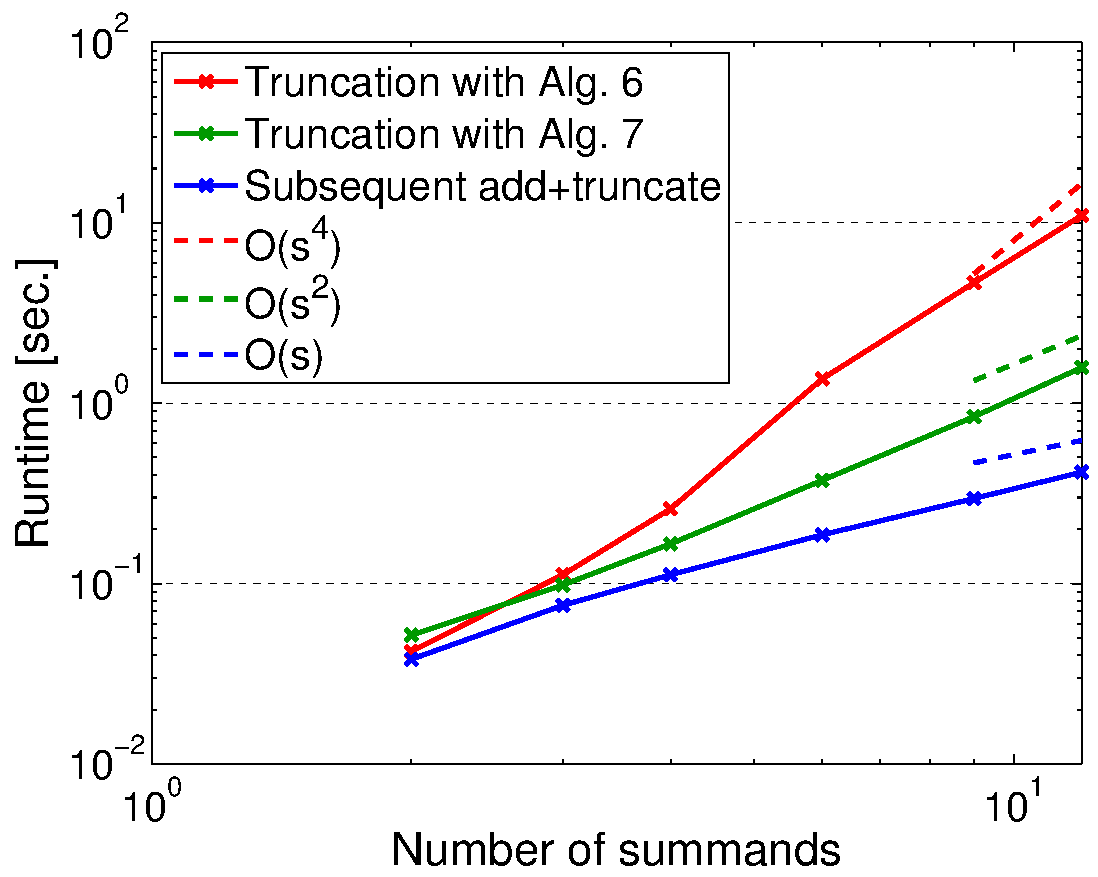
\includegraphics[width=7cm]{example_truncation.pdf}
\end{center}
\caption{Execution times for truncating a sum of tensors in HTD. Red:
Standard truncation of the sum.
Green: Truncation of the sum with using combined addition and truncation, as described in Section~\ref{sec:addtruncate}.
Blue: Successive addition and truncation, see~(\ref{eq:subsequent}).}
\label{fig:time_addtrunc}
\end{figure}

\section{Elementwise multiplication} \label{sec:elementwise}

The elementwise multiplication of two tensors is an important
operation in connection with function-related tensors and can be
performed efficiently for tensors in HTD.
In particular, this operation corresponds to the
pointwise multiplication $f(\xi_1, \ldots, \xi_d) = f_1(\xi_1, \ldots, \xi_d)
 f_2(\xi_1, \ldots, \xi_d)$ of the functions $f_1,f_2$ represented
  by the two tensors.

For illustration, we first consider
the elementwise multiplication of two low-rank matrices 
$X = U^x S^x (V^x)^H$ and
$Y = U^y S^y (V^y)^H$,
with $S^x, S^y \in \C^{r \times r}$.
Then the elementwise product (also called Hadamard product) can be written as
\begin{align*}
(X \star Y)_{i,j} &:= X_{ij} Y_{ij} = \sum_{\alpha,\beta,\gamma,\delta} U^x_{i,\alpha} U^y_{i,\gamma} S^x_{\alpha,\beta} S^y_{\gamma,\delta} V^x_{j,\beta} V^y_{j,\delta}\\
& = (U^x \odot^T U^y) (S^x \otimes S^y) (V^x \odot^T V^y)^H,
\end{align*}
where $\odot^T$ denotes a transposed variant of the Khatri-Rao product~\cite{KolB09}. More specifically,
for a matrix $A \in \C^{n \times k}$ with rows $a_j^T$ and
a matrix $B \in \C^{n \times r}$ with rows $b_j^T$, we define
\[
A \odot^T B =
\begin{bmatrix} a_1^T \\ a_2^T \\ \vdots \\ a_n^T \end{bmatrix} \odot^T
\begin{bmatrix} b_1^T \\ b_2^T \\ \vdots \\ b_n^T \end{bmatrix} :=
\begin{bmatrix} a_1^T \otimes b_1^T \\ a_2^T \otimes b_2^T \\
  \vdots \\ a_n^T \otimes b_n^T \end{bmatrix} \in \C^{n \times kr}.
\]
Note that
$A \odot^T
B = (A^T \odot B^T)^T$, where $\odot$ is the usual Khatri-Rao product.

For the elementwise multiplication of two tensors $\calX, \calY$ in HTD, the same technique
can be used to construct the leaf matrices $U_t$ and transfer tensors $\calB_t$
for an HTD of $\calX\star \calY$:
\[
U_t = U^x_t \odot^T U^y_t \text{ for leaf nodes $t$ and } \calB_t = \calB_t^x \otimes \calB_t^y \text{ for non-leaf nodes $t$},
\]
where $\otimes$ represents 
a direct generalization of 
the Kronecker product to tensors: 
For two tensors 
$\calX \in \C^{n_1 \times \cdots \times n_d},
\hat{\calX} \in \C^{\hat{n}_1 \times \cdots \times \hat{n}_d}$
we define
$(\calX \otimes \hat{\calX})_{J_1, \ldots, J_d} 
:= \calX_{i_1,\ldots,i_d} \hat{\calX}_{j_1,\ldots,j_d}$, 
with $J_\mu = (i_\mu-1) \hat{n}_\mu + j_\mu$.
%
As a consequence,
the hierarchical rank $r_t$ of $\calX \star \calY$
is the product $r^x_t r^y_t$ 
of the hierarchical ranks
of $\calX$ and $\calY$.

It would be useful
to avoid the rank growth of $\calX \star \calY$ and directly calculate
a truncated version,
similarly as for the sum of $s$ tensors 
in Section~\ref{sec:addtruncate}.
%
Unfortunately, it is not clear how to transfer the ideas from 
Section~\ref{sec:addtruncate} to the elementwise product; the Kronecker structure of the
transfer tensors does not lead in an obvious way to a reduction of computational or storage cost.
%
However, we can exploit the fact that the elementwise product
is contained in the Kronecker product. More specifically, there is
a $(0,1)$-matrix $J_n \in \R^{n^2\times n}$ with orthonormal 
columns such that
\[
a \star b = J_n^H (a \otimes b),
\]
for any two vectors $a,b\in \C^n$. This extends in a direct fashion to tensors:
\begin{equation} \label{eq:extract}
 J^H (\calX \otimes \calY) := 
(J_{n_d}^H \otimes \cdots \otimes J_{n_1}^H) (\calX \otimes \calY)
= \calX \star \calY.
\end{equation}
Hence, we can implicitly form the Kronecker product $\calX \otimes \calY$ in HTD and extract
the elementwise product after truncation.

The HTD of the Kronecker product $\calX \otimes \calY$ of two tensors $\calX, \calY$ in HTD is particularly simple:
\[ \begin{array}{rcll}
  {U}_t &:=& U_t^x \otimes U_t^y \qquad & \forall t \in \calL(\calT), \\
  {B}_t &:=& B_t^x \otimes B_t^y & \forall t \in \calN(\calT).
   \end{array}
\]
%
This implies that the reduced Gramians have Kronecker structure, $G_t = G_t^x \otimes G_t^y$,
as well as their singular value decompositions used in the standard truncation to lower rank.
Consequently, this allows for a particularly efficient HTD truncation
$\calZ$ of  $\calX \otimes \calY$. Using~(\ref{eq:extract}), the extracted tensor $J^H \calZ$ represents
an approximation of $\calX \star \calY$ satisfying the error bound
\[
\normb{\calX \star \calY - J^H \calZ}_2 
= \normb{J^H (\calX \otimes \calY - \calZ)}_2
\le \normb{\calX \otimes \calY - \calZ}_2 \le \epsilon_{abs}.
\]
Although the hierarchical ranks of $J^H \calZ$ are typically much smaller compared to $\calX \star \calY$,
the error bound above is far from being sharp.
It is therefore recommended to truncate
$J^H \calZ$ again after the extraction.

\begin{framed}\noindent
\texttt{z = x .* y} elementwise product of $\calX$ and $\calY$.\\
\texttt{z = elem\_mult(x, y, opts)} approximate elementwise product, with \texttt{opts} defined as in \texttt{truncate}.
\end{framed}

\section{HTD of linear operators on tensors} \label{sec:linop}

The use of tensors in PDE-related applications often requires the efficient storage and application
of a linear operator to tensors. In many cases, such a linear operator can be written as a short sum
of Kronecker products:
\begin{equation} \label{eq:cplikeop}
\vect(\calA(\calX)) = \sum_{j=1}^R 
\Big( A_j^{(d)} \otimes \cdots \otimes A_j^{(1)} \Big) \vect(\calX),
\quad \text{ with } A_j^{(\mu)} \in \C^{m_\mu \times n_\mu}.
\end{equation}
For example, a discretized Laplace operator in $d$ dimensions takes this form with $R = d$, see Example~\ref{example:laplace}
below. The operation~(\ref{eq:cplikeop}) can be implemented by first applying $\mu$-mode matrix products ({\tt ttm})
and then using an algorithm for computing a sum of tensors in HTD, see Section~\ref{sec:addtruncate}.
In general, this is a reasonable approach. However, for particular linear operators, a much more efficient scheme can be devised.

This scheme is based on interpreting a linear operator as a tensor, an idea which goes back
to the computational physics community~\cite{Sch11}. For example, the operator in~(\ref{eq:cplikeop})
can be vectorized into
\[
\tilde{\calA} = \sum_{j=1}^R 
\vect\Big(A_j^{(d)}\Big) \otimes \cdots \otimes \vect\Big(A_j^{(1)}\Big).
\]
Note that this format is a CP decomposition.
More generally, there is an isomorphism
\[
 \Psi: \mathfrak{L}\big(\C^{n_1 \times \cdots \times n_d }, \C^{m_1 \times \cdots \times m_d} \big) \to \C^{n_1 m_1 \times \cdots n_d m_d},
\]
which takes the matrix representation $\calA_M \in \C^{ (m_1 \cdots m_d) \times ( n_1 \cdots n_d) }$
of a linear operator $\calA$, and permutes and reshapes its entries into a tensor $\tilde \calA = \Psi(\calA)$ of order $d$.

The tensor $\tilde \calA = \Psi(\calA)$ can now be approximated in HTD by the methods described in this paper.
When applying a linear operator implicitly represented as a tensor in HTD with leaf bases $U_t^{\calA} \in \C^{m_t n_t \times s_t}$
and transfer tensors $\calB_t^{\calA}$, it is convenient to reinterpret the columns of the leaf bases as matrices $A_t^{(j)}$:
\[
 U_t^{\calA}(:,j) = \vect \big( A_t^{(j)} \big).
\]
Then the application of $\calA$ to a tensor $\calX$ of conforming size in HTD with hierarchical ranks $r_t$
again results in an HTD with 
\[
{U}_t = \Big[A^{(1)}_{t} U^x_t, \ldots, A^{(s_t)}_{t} U^x_t \Big], \quad
{\calB}_t = \calB_t^\calA \otimes \calB_t^\calX. 
\]
Hence, the hierarchical ranks grow to $s_t r_t$, which illustrates the importance of
keeping the hierarchical ranks $s_t$ of $\calA$ low.


% When taking the approximation of $\tilde{\calA}$ in HTD,
% and reversing the permutation and reshape,
% we find a matrix of the form
% \[
% \tilde{\calA} = \sum_{j_1,\ldots,j_d} \calC_{j_1,\ldots,j_d} 
% \big( A_{j_d}^{(d)} \otimes \cdots \otimes A_{j_1}^{(1)} \big).
% \]
% where $\calC$ is a tensor in HTD.
%

%
%Note that the sparsity pattern of $\calB_t^\calA$ is identical
%to the block-structure of the tensor $\calB_t$ of the resulting tensor.

The sesquilinear product
$\langle \calX, \calY \rangle_\calA$
can be computed without applying $\calA$ to one of the tensors,
by interpreting the product as a tensor network and contracting the network.
This amounts to a computational complexity of
$O(d (s n^2 r + s n r^2 + 3 s^2 r^4 + s^3 r^2))$,
where $\calX, \calY$ are in HTD with sizes $n$ and hierarchical ranks $r$, 
while $\tilde{\calA}$ is in HTD with hierarchical ranks $s$.

%leaves:
%d*s*(n^2*k + n*k^2)
%
%non-leaf nodes:
%(d-1)*(
%  s*k * k * k^2
%+ s*k * k * k^2
%+ s*k * k^2 * s*k
%+ k^2 * s^2 * s
%)
%= (d-1)*(2*s*k^4+s^2*k^4+s^3*k^2)
%Together:
%d*(s*n^2*k + s*n*k^2 + 3*s^2*k^4 + s^3*k^2)

The composition of two linear operators (i.e., the multiplication of the corresponding matrix representations)
in HTD can be calculated in a similar way as the application of a linear operator in HTD.
% of two matrices $\calA_1 \in \F^{n_1 \cdots n_d \times p_1
%  \cdots p_d}, \calA_2 \in \F^{p_1 \cdots p_d \times m_1 \cdots m_d}$ in
%
\begin{framed}\noindent
\texttt{y = apply\_mat\_to\_vec(A, x)} returns $\calY = \calA(\calX)$ for a linear operator $\calA$ in HTD.\\
\texttt{s = innerprod\_mat(x, y, A)} returns $s = \langle \calX, \calY \rangle_\calA$.\\
\texttt{C = apply\_mat\_to\_mat(A, B, p)} returns $\calC = \calA \circ \calB$ for two linear operators
$\calA \in \mathfrak{L}\big(\C^{p_1 \times \cdots \times p_d }, \C^{n_1 \times \cdots \times n_d} \big)$
and $\calB \in \mathfrak{L}\big(\C^{m_1 \times \cdots \times m_d }, \C^{p_1 \times \cdots \times p_d} \big)$.
\end{framed}
%
Note that a truncation of a linear operator $\calA$ to HTD produces a quasi-optimal approximation in the Frobenius norm.
Therefore, its effect on the smallest eigenvalues of $\calA$ is likely to be significant and its use for the direct
solution of linear systems questionable.
%
However, 
this approximation may still be useful
in the construction of preconditioners,
and there are some notable cases
for which an exact representation in HTD of low rank is possible.

\begin{example} \label{example:laplace}
A discretized Laplace-like operator of the form
\begin{equation} \label{eq:lapl}
A^{(d)} \otimes I \otimes \cdots \otimes I 
\  + \   I \otimes A^{(d-1)} \otimes I \otimes \cdots \otimes I 
\  + \  \cdots
\  + \  I \otimes \cdots \otimes I \otimes A^{(1)}
\end{equation}
can be represented exactly in HTD with hierarchical rank $2$ for any dimension tree $\calT$:
\[
U_t = \big[ \vect(I), \vect(A^{(t)}) \big] \quad \forall t \in \calL(\calT)
\]
\[B_t = \left[ \begin{array}{cc}
1 & 0 \\ 0 & 1 \\ 0 & 1 \\ 0 & 0
\end{array} \right] \quad \forall t \in \calN(\calT) \setminus \{t_{\text{root}}\},\qquad 
 B_{t_{\text{root}}} =
\left[ \begin{array}{c}
0 \\ 1 \\ 1 \\ 0
\end{array} \right].
\]
A similar decomposition has been proposed for the TT decomposition in \cite{KazK10}.
\end{example}

\section{Examples} \label{sec:examples}

In the following, we will show two examples for the use of the 
described \htucker{} toolbox. One relatively simple example is concerned with a
tensor containing function samples, and another example is concerned with a tensor
containing solutions to a parameter-dependent partial differential equation.

\begin{example} \rm \label{example:sum_reciproc}
The tensor $\calX$ is defined to contain all function values of the $d$-variate
function
\[
f(\xi_1, \ldots, \xi_d) = \frac{1}{\xi_1 + \cdots + \xi_d}
\]
on a uniform tensor grid in $[1,10]^d$.
The following commands create this tensor as a standard {\sc Matlab}
multidimensional array (see \texttt{examples/example\_sum\_reciproc.m}):
\begin{framed} \small
\noindent
\vspace{-3ex}
\begin{verbatim}
n = 50; d = 4;
xi = linspace(1, 10, n)';
xil = xi*ones(1, n^(d-1)); xil = reshape(xil, n*ones(1, d));
xisum = xil;
for ii=2:d
  xisum = xisum + permute(xil, [ii, 2:ii-1, 1, ii+1:d]);
end
x = 1./xisum;
\end{verbatim}\vspace{-2ex}
\end{framed}
\noindent We then truncate this full tensor $\calX$ to HTD:
\begin{framed}\small \noindent 
\vspace{-3ex} 
\begin{verbatim}
opts.max_rank = 10;  opts.rel_eps = 1e-5;
x_ht = truncate(x, opts);
rel_err = norm(x(:) - x_ht(:))/norm(x(:))
> 1.3403e-06
\end{verbatim}\vspace{-2ex}
\end{framed}
\noindent Note that this approach is limited to small values of $d$, as
$\calX$ is constructed explicitly. An alternative approach relies on the
following identity
\[
\frac{1}{\xi_1+\cdots+\xi_d} 
= \int_0^\infty \exp(-t\cdot(\xi_1+\cdots+\xi_d)) dt 
\approx \sum_{j=-M}^M \omega_j \prod_{\mu=1}^d e^{-\alpha_j \xi_\mu}.
\]
Suitable coefficients $\alpha_j, \omega_j$ are described in \cite{Gra04a,Hac08}.
Sampling the function on the right-hand side directly results in a CP decomposition of rank
$2M+1$. This can then be converted to the HTD format, where it can be
truncated further, resulting in much smaller ranks; from tensor rank $51$ to
hierarchical rank $5$ in our example:
\begin{framed}\small \noindent \vspace{-3ex} 
\begin{verbatim}
M = 25; j = (-M:M);
xMin = d*min(xi);
hst = pi/sqrt(M);
alpha = -2*log(exp(j*hst)+sqrt(1+exp(2*j*hst)))/xMin;
omega = 2*hst./sqrt(1+exp(-2*j*hst))/xMin;

x_cp = cell(1, d);
for ii=1:d, x_cp{ii} = exp(xi*alpha); end
x_cp{1} = x_cp{1}*diag(omega);
x_cp = htensor(x_cp);
rel_err = norm(x(:) - x_cp(:))/norm(x(:))
> 1.4848e-06
x_trunc_cp = truncate(x_cp, opts);
rel_err = norm(x(:) - x_trunc_cp(:))/norm(x(:))
> 2.0001e-06
\end{verbatim}\vspace{-1ex}
\end{framed}
The approach above is limited to functions of a very
specific structure. A more generally applicable method relies on a
Newton-Schultz iteration for finding the elementwise reciprocal of a
tensor in HTD, see \texttt{examples/elem\_reciprocal.m}
in the \htucker{} toolbox. In the context of low-rank tensors, such an iteration was
already proposed by Oseledets in \cite{tttoolboxv1}.
\begin{framed}\small \noindent
\textbf{Construction of $\calX$ using Newton-Schulz iteration}\\
\vspace{-3ex} 
\begin{verbatim}
xisum_cp = cell(1, d);
for ii=1:d
  xisum_cp{ii} = ones(n, d); xisum_cp{ii}(:, ii) = xi;
end

opts.elem_mult_max_rank = 50; opts.elem_mult_abs_eps = 1e-2;
opts.max_rank = 50; opts.rel_eps = 1e-5;
x0 = htenones(size(x)) / ( d*max(xi) );
x_rec = elem_reciprocal(htensor(xisum_cp), opts, x0 );
rel_err = norm(x(:) - x_rec(:))/norm(x(:))
> 1.3595e-06
\end{verbatim}\vspace{-1ex}
\end{framed}
Note that, independent of the choice of the three methods above, the obtained
\texttt{htensor} objects \texttt{x\_ht}, \texttt{x\_trunc\_cp}, \texttt{x\_rec} all have hierarchical ranks $5$, and very similar singular value decay (see Figure~\ref{fig:example_sv}).
\begin{figure}
\begin{center}
  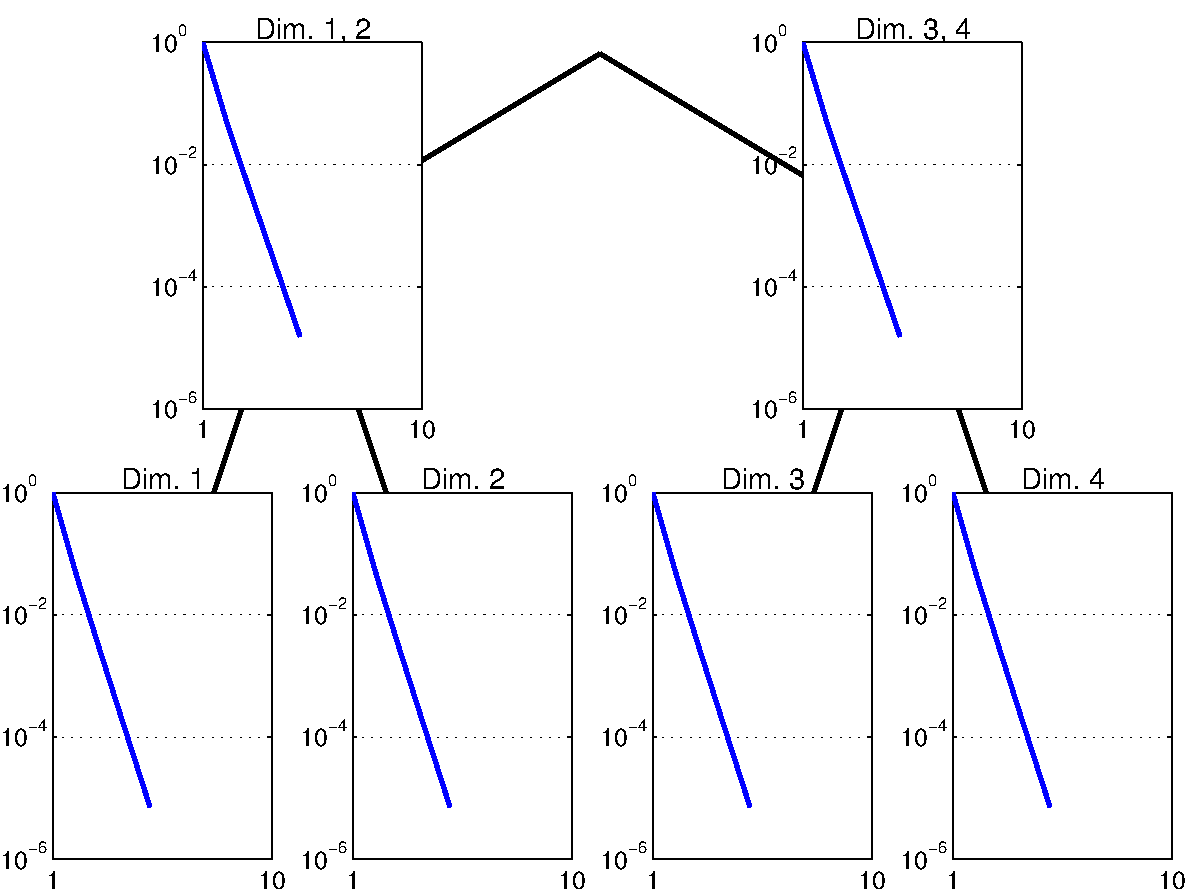
\includegraphics[width=9cm]{example_sv}
\end{center}
\caption{Singular value tree of tensors \texttt{x\_ht}, \texttt{x\_trunc\_cp}, \texttt{x\_rec} in HTD (Example~\ref{example:sum_reciproc}), produced by the function \texttt{plot\_sv}.} 
\label{fig:example_sv}
\end{figure}
Having obtained an approximation of the sampled tensor through any of
the methods described above, we will now show how to use this approximation to evaluate an integral of the form
\[
\int_1^{10} \cdots \int_1^{10} \frac{1}{\xi_1 + \cdots + \xi_d} \text{d}\xi_1 \cdots \text{d}\xi_d.
\]
We use Simpson's rule in each variable to perform numerical quadrature on the tensor grid.
%Note that other quadrature rules can be used,
%by sampling a tensor on the respective nodes.
\begin{framed}\small \noindent
\textbf{Quadrature using approximation in HTD}\\
\vspace{-3ex} 
\begin{verbatim}
% Construction of quadrature weights 
h = 9/(n-1);
w = 4*ones(n, 1); w(3:2:end-2) = 2;  w(1) = 1;  w(end) = 1;
w = h/3*w;

% Inner product between weights and function values by repeated contraction
for ii=1:d, w_cell{ii} = w; end
ttv(x_ht, w_cell)
\end{verbatim} 
\vspace{-2ex}
\end{framed}
\hfill $\diamond$
\end{example}

\begin{example} \rm
  \label{example:cookies}
In the following, we consider an example from~\cite{KreT10b}
concerning the solution of parameter-dependent linear systems.
More specifically, let $x(\alpha)$ with $\alpha = (\alpha_1,\alpha_2,\alpha_3,\alpha_4)$ denote the solution of
\begin{equation} \label{eq:paramsys}
\left(A_0 + \sum_{\mu=1}^4 \alpha_\mu A_\mu\right) \, x(\alpha) = b.
\end{equation}
Then we take $m$ samples $\{ \alpha^{(\mu)}_1, \ldots, \alpha^{(\mu)}_m \}$ for each parameter $\alpha_{\mu}$ and stack the sampled solutions into
a ``snapshot'' tensor $\calX \in \R^{n \times m \times m \times m \times m}$ as follows:
\[
 \calX(:, i_1, i_2, i_3, i_4) = x\Big(\alpha^{(1)}_{i_1}, \alpha^{(2)}_{i_2}, \alpha^{(3)}_{i_3}, \alpha^{(4)}_{i_4} \Big), \qquad i_\mu = 1,\ldots,m.
\]
As explained in~\cite{KreT10b}, this tensor can be interpreted as the solution of a (huge) symmetric positive definite linear system $\calA(\calX) = \calB$. This allows us to approximate the solution in HTD
by applying a low-rank variant of the preconditioned CG
method to $\calA(\calX) = \calB$, see \texttt{examples/cg\_tensor.m}.

Our specific example from \cite[Sec. 4]{KreT10b} is the stationary heat equation on a square domain with Dirichlet boundary conditions. The heat conductivity coefficient $\sigma(\xi)$ is piecewise constant and depends on the four parameters as follows:
\[
\sigma(\xi) = 
\left\{ \begin{array}{cl}
1 + \alpha_\mu  & \text{ for } \xi \in \Omega_\mu,\ \mu = 1,\ldots, 4,\\
1             & \text{ for } \xi \notin \bigcup_{\mu=1}^4 \Omega_\mu,
\end{array} \right.
\]
where $\Omega_1, \ldots, \Omega_4$ are mutually disjoint discs inside
the domain. A finite element discretization results in a
parameter-dependent linear system~(\ref{eq:paramsys}) of size $n =
1580$. We choose the samples $\{ \alpha^{(\mu)}_1, \ldots,
\alpha^{(\mu)}_m \} = \{ 0, 1, \ldots, 100 \}$ and hence $m =
101$. The matrices $A_0, \ldots, A_4$ as well as the vector $b$ are contained in the file \texttt{examples/cookies\_matrices\_2x2.mat}, and the following code can be found in \texttt{examples/example\_cookies.m}.
\begin{framed}\small \noindent
\vspace{-3ex} 
\begin{verbatim}
load cookies_matrices_2x2
A_handle = handle_lin_mat(A, {[], 0:100, 0:100, 0:100, 0:100});
M_handle = handle_inv_mat(A{1});
e = ones(101, 1); b_cell = {b, e, e, e, e};
b_tensor = htensor(b_cell);

opts.max_rank = 30;   opts.rel_eps = 1e-10;
opts.maxit = 50;      opts.tol = 0;
[x, norm_r] = cg_tensor(A_handle, M_handle, b_tensor, opts);
\end{verbatim}
\vspace{-2ex} 
\end{framed}

\noindent From the resulting tensor $\calX \in \R^{1580 \times 101 \times 101 \times 101 \times 101}$, we calculate the sample mean and variance of $x$, see also Figure~\ref{fig:cookies_mean_var}.
\begin{framed}\small \noindent
\vspace{-3ex} 
\begin{verbatim}
x_mean = full(ttv(x, {e,e,e,e}, [2 3 4 5])) / 101^4;
x_diff = x - htensor({x_mean,e,e,e,e});
x_var = diag(full(ttt(x_diff, x_diff, [2 3 4 5]))) / ( 101^4 - 1 );
\end{verbatim}
\vspace{-2ex} 
\end{framed}
\begin{figure}
\begin{center}
  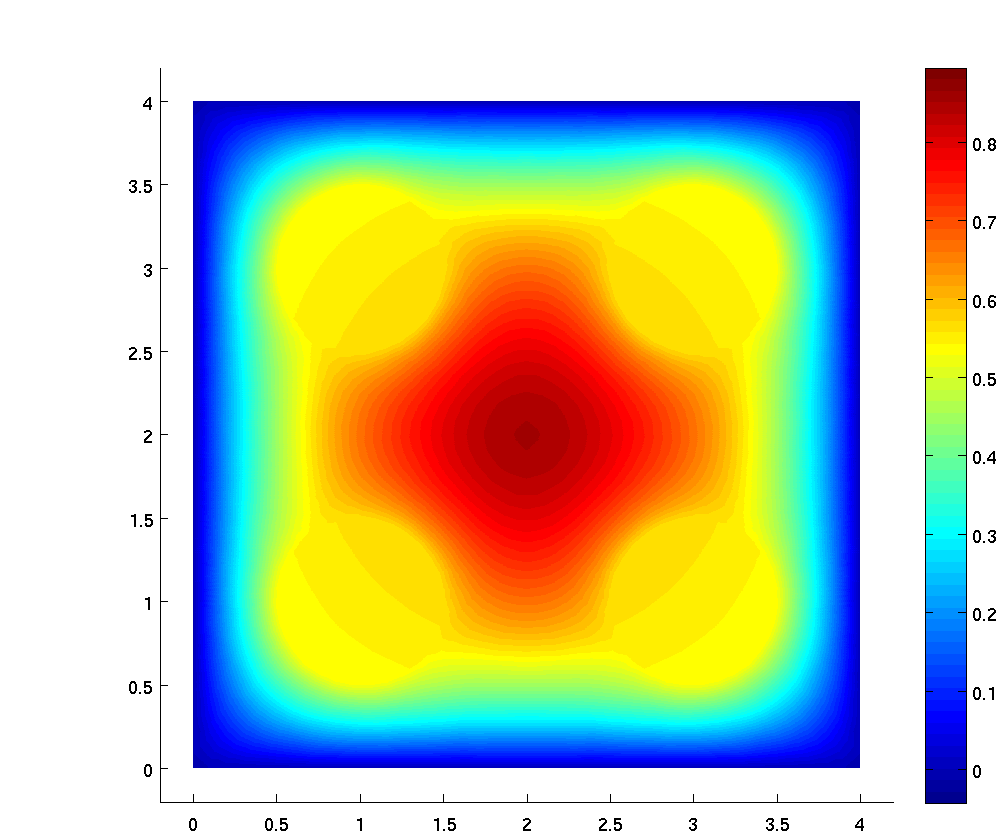
\includegraphics[width=7cm]{cookies_mean}
$\qquad$
  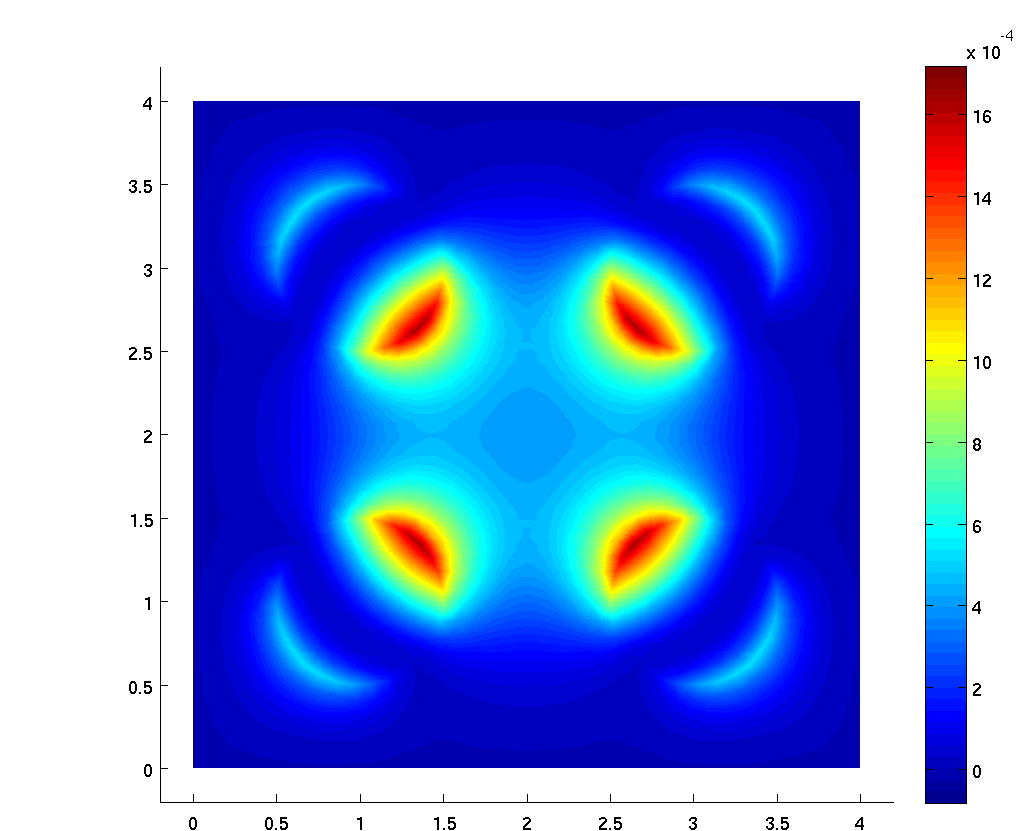
\includegraphics[width=7cm]{cookies_var}
\end{center}
\caption{Sample mean and variance of the parameter-dependent stationary heat equation (Example~\ref{example:cookies}).} 
\label{fig:cookies_mean_var}
\end{figure}
\hfill $\diamond$
\end{example}

\section{Conclusions and ongoing work}

The main goal of this work was to provide a convenient way to work with tensors in HTD.
Several extensions of this work are possible and currently under consideration.

The most expensive operations of the \htucker{} toolbox are typically calls to level
$3$ BLAS and LAPACK functions, and hence there is a simple to gain performance by, e.g., linking
to multi-threaded BLAS. However, in order to address challenging
applications that feature high ranks, there is clearly a need
for a more advanced implementation fine-tuned to modern high-performance and
parallel machines.

One of the most challenging aspects in using low-rank tensor decompositions, such as HTD,
is the a priori choice of a suitable decomposition. This also includes the choice of the
dimension tree in HTD, which at the moment is ad hoc. The development of rational criteria or
effective heuristics for these choices is an important open question.

The work on low-rank tensor decompositions is quickly expanding. As new methods emerge
and mature, they will be added to future versions of the \htucker{} toolbox.
Candidates include dynamical low-rank methods for HTD~\cite{Arnold2012,Lubich2012} and 
low-rank tensor cross approximation for HTD~\cite{Ballani2012c,Ballani2012a}. For both, preliminary implementations are already available
see~\url{http://anchp.epfl.ch/htucker}.

\begin{thebibliography}{10}

\bibitem{AcaDK11}
E.~Acar, D.~M. Dunlavy, and T.~G. Kolda.
\newblock A scalable optimization approach for fitting canonical tensor
  decompositions.
\newblock {\em J. Chemometrics}, 25(2):67--86, 2011.

\bibitem{AndB00}
C.~A. Andersson and R.~Bro.
\newblock The {$N$-way} toolbox for {MATLAB}.
\newblock {\em Chemometrics and Intelligent Laboratory Systems}, 52(1):1--4,
  2000.
\newblock Available from \url{http://www.models.life.ku.dk/nwaytoolbox}.

\bibitem{Arnold2012}
A.~Arnold and T.~Jahnke.
\newblock On the approximation of high-dimensional differential equations in
  the hierarchical {T}ucker format.
\newblock Technical report, KIT, Karlsruhe, Germany, 2012.

\bibitem{BadK06}
B.~W. Bader and T.~G. Kolda.
\newblock Algorithm 862: {MATLAB} tensor classes for fast algorithm
  prototyping.
\newblock {\em ACM Trans. Math. Software}, 32(4):635--653, 2006.
\newblock Available from
  \url{http://csmr.ca.sandia.gov/~tgkolda/TensorToolbox/}.

\bibitem{BadK07}
B.~W. Bader and T.~G. Kolda.
\newblock Efficient {MATLAB} computations with sparse and factored tensors.
\newblock {\em SIAM J. Sci. Comput.}, 30(1):205--231, 2007.

\bibitem{Ballani2012c}
J.~Ballani.
\newblock {\em {Fast evaluation of near-field boundary integrals using tensor
  approximations}}.
\newblock Dissertation, Universit\"at Leipzig, 2012.

\bibitem{BalG10}
J.~Ballani and L.~Grasedyck.
\newblock A projection method to solve linear systems in tensor format.
\newblock {\em Numer. Linear Algebra Appl.}, 20(1):27--43, 2013.

\bibitem{Ballani2012a}
J.~Ballani, L.~Grasedyck, and M.~Kluge.
\newblock Black box approximation of tensors in hierarchical {T}ucker format.
\newblock Technical report, RWTH Aachen, Germany, 2012.
\newblock To be published, available at
  \url{http://dx.doi.org/10.1016/j.laa.2011.08.010}.

\bibitem{Bau11}
B.~{Bauer et al.}
\newblock The {ALPS} project release 2.0: open source software for strongly
  correlated systems.
\newblock {\em J. Stat. Mech.}, 5, 2011.

\bibitem{CarC70}
J.~Carroll and J.-J. Chang.
\newblock Analysis of individual differences in multidimensional scaling via an
  n-way generalization of {"Eckart-Young"} decomposition.
\newblock {\em Psychometrika}, 35:283--319, 1970.

\bibitem{DeLDV00}
L.~De~Lathauwer, B.~De~Moor, and J.~Vandewalle.
\newblock A multilinear singular value decomposition.
\newblock {\em SIAM J. Matrix Anal. Appl.}, 21(4):1253--1278, 2000.

\bibitem{Espig2012d}
M.~Espig and W.~Hackbusch.
\newblock A regularized {N}ewton method for the efficient approximation of
  tensors represented in the canonical tensor format.
\newblock {\em Numer. Math.}, 122(3):489--525, 2012.

\bibitem{EspHHS11}
M.~Espig, W.~Hackbusch, S.~Handschuh, and R.~Schneider.
\newblock Optimization problems in contracted tensor networks.
\newblock {\em Computing and Visualization in Science}, 14:271--285, 2011.

\bibitem{Espig2012e}
M.~Espig, W.~Hackbusch, T.~Rohwedder, and R.~Schneider.
\newblock Variational calculus with sums of elementary tensors of fixed rank.
\newblock {\em Numer. Math.}, 122(52):469--488, 2012.

\bibitem{tensorcalculus}
M.~Espig, M.~Schuster, A.~Killaitis, N.~Waldren, P.~W\"ahnert, S.~Handschuh,
  and H.~Auer.
\newblock {TensorCalculus library}, 2012.
\newblock Available from \url{http://gitorious.org/tensorcalculus}.

\bibitem{GolV96}
G.~H. Golub and C.~F. Van~Loan.
\newblock {\em Matrix Computations}.
\newblock Johns Hopkins University Press, Baltimore (MD), third edition, 1996.

\bibitem{Gra04a}
L.~Grasedyck.
\newblock Existence and computation of low {K}ronecker-rank approximations for
  large linear systems of tensor product structure.
\newblock {\em Computing}, 72(3-4):247--265, 2004.

\bibitem{Gra10summer}
L.~Grasedyck.
\newblock Hierarchical low rank approximation of tensors and multivariate
  functions, 2010.
\newblock Lecture notes of Z\"urich summer school on "Sparse Tensor
  Discretizations of High-Dimensional Problems".

\bibitem{Gra10}
L.~Grasedyck.
\newblock Hierarchical singular value decomposition of tensors.
\newblock {\em SIAM J. Matrix Anal. Appl.}, 31(4):2029--2054, 2010.

\bibitem{Hac08}
W.~Hackbusch.
\newblock Approximation of $1/x$ by exponential sums.
\newblock Available from
  \url{http://www.mis.mpg.de/scicomp/EXP_SUM/1_x/tabelle}. Retrieved August
  2008.

\bibitem{Hac12}
W.~Hackbusch.
\newblock {\em Tensor Spaces and Numerical Tensor Calculus}.
\newblock Springer, 2012.

\bibitem{HacKST08}
W.~Hackbusch, B.~N. Khoromskij, S.~A. Sauter, and E.~E. Tyrtyshnikov.
\newblock Use of tensor formats in elliptic eigenvalue problems.
\newblock {\em Numer. Linear Algebra Appl.}, 19(1):133--151, 2012.

\bibitem{HacK09}
W.~Hackbusch and S.~K{\"u}hn.
\newblock A new scheme for the tensor representation.
\newblock {\em J. Fourier Anal. Appl.}, 15(5):706--722, 2009.

\bibitem{Har70}
R.~A. Harshman.
\newblock Foundations of the {PARAFAC} procedure: Models and conditions for an
  "explanatory" multi-modal factor analysis.
\newblock {\em {UCLA} Working Papers in Phonetics}, 16:1--84, 1970.

\bibitem{HolRS10b}
S.~Holtz, T.~Rohwedder, and R.~Schneider.
\newblock The alternating linear scheme for tensor optimization in the {T}ensor
  {T}rain format.
\newblock {\em SIAM J. Sci. Comput.}, 34(2):A683--A713, 2012.

\bibitem{Huckle2013}
T.~Huckle, K.~Waldherr, and T.~Schulte-Herbr{\"u}ggen.
\newblock Computations in quantum tensor networks.
\newblock {\em Linear Algebra Appl.}, 438(2):750--781, 2013.

\bibitem{KazK10}
V.~A. Kazeev and B.~N. Khoromskij.
\newblock Low-rank explicit {QTT} representation of {Laplace} operator and its
  inverse.
\newblock {\em SIAM J. Matrix Anal. Appl.}, 33(3):742--758, 2012.

\bibitem{KhoO10}
B.~N. Khoromskij and I.~V. Oseledets.
\newblock Quantics-{TT} collocation approximation of parameter-dependent and
  stochastic elliptic {PDEs}.
\newblock {\em Comput. Methods Appl. Math.}, 10(4):376--394, 2010.

\bibitem{KhoO09}
B.~N. Khoromskij and I.~V. Oseledets.
\newblock {QTT} approximation of elliptic solution operators in higher
  dimensions.
\newblock {\em Russian J. Numer. Anal. Math. Modelling}, 26(3):303--322, 2011.

\bibitem{KhoS10}
B.~N. Khoromskij and Ch. Schwab.
\newblock Tensor-structured {G}alerkin approximation of parametric and
  stochastic elliptic {PDEs}.
\newblock {\em SIAM J. Sci. Comput.}, 33(1):364--385, 2011.

\bibitem{KocL10}
O.~Koch and C.~Lubich.
\newblock Dynamical tensor approximation.
\newblock {\em SIAM J. Matrix Anal. Appl.}, 31(5):2360--2375, 2010.

\bibitem{KolB09}
T.~G. Kolda and B.~W. Bader.
\newblock Tensor decompositions and applications.
\newblock {\em SIAM Review}, 51(3):455--500, 2009.

\bibitem{KreT10}
D.~Kressner and C.~Tobler.
\newblock Krylov subspace methods for linear systems with tensor product
  structure.
\newblock {\em SIAM J. Matrix Anal. Appl.}, 31(4):1688--1714, 2010.

\bibitem{KreT10b}
D.~Kressner and C.~Tobler.
\newblock Low-rank tensor {K}rylov subspace methods for parametrized linear
  systems.
\newblock {\em SIAM J. Matrix Anal. Appl.}, 32(4):1288--1316, 2011.

\bibitem{Lubich2012}
Ch. Lubich, T.~Rohwedder, R.~Schneider, and B.~Vandereycken.
\newblock Dynamical approximation of hierarchical {T}ucker and tensor-train
  tensors.
\newblock Technical report, July 2012.

\bibitem{tttoolboxv1}
I.~V. Oseledets.
\newblock {MATLAB TT-Toolbox Version 1.0}, May 2009.
\newblock See \url{http://spring.inm.ras.ru/osel/?page_id=24}.

\bibitem{tttoolbox}
I.~V. Oseledets.
\newblock {MATLAB TT-Toolbox Version 2.1}, May 2011.
\newblock See \url{http://spring.inm.ras.ru/osel/?page_id=24}.

\bibitem{Osel09}
I.~V. Oseledets.
\newblock Tensor-train decomposition.
\newblock {\em SIAM J. Sci. Comput.}, 33(5):2295--2317, 2011.

\bibitem{OseK10}
I.~V. Oseledets and B.~N. Khoromskij.
\newblock {DMRG+QTT} approach to high-dimensional quantum molecular dynamics.
\newblock Preprint 69/2010, Max-Planck-Institut f\"ur Mathematik in den
  Naturwissenschaften, 2010.

\bibitem{Sch11}
U.~Schollw\"ock.
\newblock The density-matrix renormalization group in the age of matrix product
  states.
\newblock {\em Annals of Physics}, 326, 2011.

\bibitem{Tob12}
C.~Tobler.
\newblock {\em Low-rank Tensor Methods for Linear Systems and Eigenvalue
  Problems}.
\newblock PhD thesis, ETH Z{\"u}rich, Switzerland, 2012.

\bibitem{Tucker66}
L.~Tucker.
\newblock Some mathematical notes on three-mode factor analysis.
\newblock {\em Psychometrika}, 31:279--311, 1966.

\end{thebibliography}

\begin{preprint}
\appendix

\newpage
\section{List of {\sc Matlab} functions} \label{sec:functionality}

Tables \ref{tab:htucker_functions1}, \ref{tab:htucker_functions2}, and~\ref{tab:htucker_functions3}
give an overview of the complete functionality of our {\sc Matlab} toolbox \htucker. More details
for the use of each function can be obtained using the command {\tt help}.

\begin{table}[h] \small
  \begin{tabular}{|p{3.2cm}|p{11cm}|}
\hline 
\multicolumn{2}{|c|}{Construction of \texttt{htensor} objects.} \\
\hline 
\texttt{htensor}            & Construct a tensor in HTD and return {\tt htensor} object.\\
\texttt{define\_tree}       & Define dimension tree.\\
\hline \hline
\multicolumn{2}{|c|}{Basic functionality} \\
\hline
\texttt{cat}                & Concatenate two {\tt htensor} objects.\\
\texttt{change\_dimtree}    & Change dimension tree of htensor.\\
\texttt{change\_root}       & Change root of the dimension tree.\\
\texttt{check\_htensor}     & Check internal consistency of {\tt htensor}.\\
\texttt{conj}               & Complex conjugate of {\tt htensor}.\\
\texttt{disp}               & Command window display of dimension tree of {\tt htensor}.\\
\texttt{display}            & Command window display of dimension tree of {\tt htensor}.\\
\texttt{disp\_all}          & Command window display of {\tt htensor}.\\
\texttt{end}                & Last index in one mode of {\tt htensor}.\\
\texttt{equal\_dimtree}     & Compare dimension trees of two {\tt htensor} objects.\\
\texttt{full}               & Convert {\tt htensor} to a (full) tensor.\\
\texttt{full\_block}        & Return subblock of {\tt htensor} as a (full) tensor.\\
\texttt{full\_leaves}        & Convert leaf matrices $U_t$ to dense matrices. \\
\texttt{ipermute}           & Inverse permute dimensions of {\tt htensor}.\\
\texttt{isequal}            & Check whether two htensors are equal.\\
\texttt{mrdivide (/)}       & Scalar division for {\tt htensor}.\\
\texttt{mtimes (*)}         & Scalar multiplication for {\tt htensor}.\\
\texttt{ndims}              & Order (number of dimensions) of {\tt htensor}.\\
\texttt{ndofs}              & Number of degrees of freedom in {\tt htensor}.\\
\texttt{norm}               & Norm of {\tt htensor}.\\
\texttt{norm\_diff}         & Norm of difference between {\tt htensor} and full tensor.\\
\texttt{nvecs}              & Dominant left singular vectors for matricization of {\tt htensor}.\\
\texttt{permute}            & Permute dimensions of {\tt htensor}.\\
\texttt{plot\_sv}           & Plot singular value tree of {\tt htensor}.\\
\texttt{rank}               & Hierarchical ranks of {\tt htensor}.\\
\texttt{singular\_values}   & Singular values for matricizations of {\tt htensor}.\\
\texttt{size}               & Size of {\tt htensor}.\\
\texttt{sparse\_leaves}      & Convert leaf matrices $U_t$ to sparse matrices. \\
\texttt{spy}                & Plot sparsity pattern of the nodes of {\tt htensor}.\\
\texttt{squeeze}            & Remove singleton dimensions from {\tt htensor}.\\
\texttt{subsasgn}           & Subscripted assignment for {\tt htensor}.\\
\texttt{subsref}            & Subscripted reference for {\tt htensor}.\\
\texttt{subtree}            & Return all nodes in the subtree of a node.\\
\texttt{uminus}             & Unary minus (-) of {\tt htensor}.\\
\texttt{uplus}              & Unary plus for {\tt htensor}.\\
\hline 
\end{tabular}
  \caption{List of functions in \htucker{} toolbox (part 1).} \label{tab:htucker_functions1}
\end{table}

\begin{table} \small
  \begin{tabular}{|p{3.2cm}|p{11cm}|}
\hline
\multicolumn{2}{|c|}{Operations with \texttt{htensor} objects.} \\
\hline
\texttt{elem\_mult}         & Approximate element-by-element multiplication for {\tt htensor}.\\
\texttt{innerprod}          & Inner product for {\tt htensor}.\\
\texttt{minus (-)}          & Binary subtraction for {\tt htensor}.\\
\texttt{plus (+)}           & Binary addition for {\tt htensor}.\\
\texttt{power (.\^{}2)}     & Element-by-element square for {\tt htensor}.\\
\texttt{times (.*)}         & Element-by-element multiplication for {\tt htensor}.\\
\texttt{ttm}                & $N$-mode multiplication of {\tt htensor} with matrix.\\
\texttt{ttt}                & Tensor-times-tensor for {\tt htensor}.\\
\texttt{ttv}                & Tensor-times-vector for {\tt htensor}.\\
\hline \hline
\multicolumn{2}{|c|}{Orthogonalization and truncation.} \\
\hline
\texttt{gramians}           & Reduced Gramians of {\tt htensor} in orthogonalized HTD.\\
\texttt{gramians\_cp}       & Reduced Gramians of CP tensor.\\
\texttt{gramians\_nonorthog} & Reduced Gramians of {\tt htensor}.\\
\texttt{gramians\_sum}      & Reduced Gramians for sum of {\tt htensor} objects.\\
\texttt{left\_svd\_gramian} & Left singular vectors and values from Gramian.\\
\texttt{left\_svd\_qr}      & Left singular vectors and values.\\
\texttt{orthog}             & Orthogonalize HTD of {\tt htensor}.\\
\texttt{trunc\_rank}        & Return rank according to user-specified parameters.\\
\texttt{truncate}            & Truncate full tensor/{\tt htensor}/CP to {\tt htensor}.\\
\texttt{truncate\_cp}       & Truncate CP tensor to lower-rank {\tt htensor}. \\
\texttt{truncate\_ltr}      & Truncate full tensor to {\tt htensor}, leaves-to-root.\\
\texttt{truncate\_nonorthog} & Truncate {\tt htensor} to lower-rank {\tt htensor}.\\
\texttt{truncate\_rtl}      & Truncate full tensor to {\tt htensor}, root-to-leaves.\\
\texttt{truncate\_std}       & Truncate {\tt htensor} to lower-rank {\tt htensor}.\\
\texttt{truncate\_sum}      & Truncate sum of {\tt htensor} objects to lower-rank {\tt htensor}.
.\\
\hline \hline
\multicolumn{2}{|c|}{Linear Operators.} \\
\hline
\texttt{apply\_mat\_to\_mat}& Applies an operator in HTD to another operator in HTD. \\
\texttt{apply\_mat\_to\_vec}& Applies an operator in HTD to {\tt htensor}.\\
\texttt{full\_mat}          & Full matrix represented by an operator in HTD.\\
\texttt{innerprod\_mat}     & Weighted inner product for {\tt htensor}.\\
\hline \hline
\multicolumn{2}{|c|}{Interface with Tensor Toolbox.} \\
\hline
\texttt{ktensor\_approx}    & Approximation of {\tt htensor} by {\tt ktensor}.\\
\texttt{mttkrp}             & Building block for approximating {\tt htensor} by {\tt ktensor}.\\
\texttt{ttensor}            & Convert {\tt htensor} to a Tensor Toolbox ttensor.\\
\hline
\end{tabular}
  \caption{List of functions in \htucker{} toolbox (part 2).} \label{tab:htucker_functions2}
\end{table}

\begin{table} \small
\begin{tabular}{|p{4.4cm}|p{9.8cm}|}
 \hline
\multicolumn{2}{|c|}{Auxiliary functions for full tensors.} \\
\hline
\texttt{dematricize}        & Determine (full) tensor from matricization.\\
\texttt{diag3d}             & Return third-order diagonal tensor.\\
\texttt{isindexvector}      & Check whether input is index vector.\\
\texttt{khatrirao\_aux}     & Khatri-Rao product.\\
\texttt{khatrirao\_t}       & Transposed Khatri-Rao product.\\
\texttt{matricize}          & Matricization of (full) tensor.\\
\texttt{spy3}               & Plot sparsity pattern of order-$3$ tensor.\\
\texttt{ttm}                & $N$-mode multiplication of (full) tensor with matrix.\\
\texttt{ttt}                & Tensor times tensor (full tensors).\\
%\hline \hline
%\multicolumn{2}{|c|}{Test.} \\
%\hline
%\texttt{test\_functions}           & Simple test script to check for obvious bugs.\\
\hline \hline
\multicolumn{2}{|c|}{Example tensors.} \\
\hline
\texttt{gen\_invlaplace}     & htensor for approx. inverse of Laplace-like matrix.\\
\texttt{gen\_laplace}        & {\tt htensor} for Laplace-like matrix.\\
\texttt{gen\_sin\_cos}       & Function-valued {\tt htensor} for sine and cosine.\\
\texttt{htenones}           & {\tt htensor} with all elements one.\\
\texttt{htenrandn}          & Random {\tt htensor}.\\
\texttt{laplace\_core}       & Core tensor for Laplace operator.\\
\texttt{reciproc\_sum}             & Function-valued tensor for $1/(\xi_1 + \cdots + \xi_d)$.\\
\hline \hline
\multicolumn{2}{|c|}{Examples} \\
\hline
\texttt{cg\_tensor}             & Truncated Conjugate Gradient method for htensor.\\
\texttt{demo\_basics}           & Demonstration of basic htensor functionality.\\
\texttt{demo\_constructor}      & Demonstration of htensor constructors.\\
\texttt{demo\_elem\_reciprocal} & Demonstration of element-wise reciprocal.\\
\texttt{demo\_function}         & Demonstration of htensor function approximation.\\
\texttt{demo\_invlaplace}       & Demonstration of approximate inverse Laplace.\\
\texttt{demo\_operator}         & Demonstration of operator-HTD format.\\
\texttt{elem\_reciprocal}       & Iterative computation of elementwise reciprocal for htensor.\\
\texttt{example\_cancellation}  & Cancellation in $\tan(x) + 1/x - \tan(x)$.\\
\texttt{example\_cancellation2} & Cancellation in $\exp(-x^2) + \sin(x)^2 + \cos(x)^2$.\\
\texttt{example\_cookies}       & Apply CG method to a parametric PDE.\\
\texttt{example\_maxest}        & Example for computing element of maximal absolute value.\\
\texttt{example\_spins}         & Demonstration of operator-HTD for 1D spin system.\\
\texttt{example\_sum\_reciproc} & Apply element-wise reciprocal method to sum of tensors.\\
\texttt{example\_truncation}    & Comparison of speed for different truncation methods.\\
\texttt{handle\_inv\_mat}       & Function handle to Kronecker structured matrix multiplication.\\
\texttt{handle\_lin\_mat}       & Function handle to Kronecker structured matrix multiplication.\\
\texttt{maxest}                 & Approximate element of maximal absolute value.\\
\hline
\end{tabular}
  \caption{List of functions in \htucker{} toolbox (part 3).} \label{tab:htucker_functions3}
%\caption{List of examples in \htucker{} toolbox.} \label{tab:htucker_functions3}
\end{table}


\newpage
\section{Proofs of approximation results} \label{sec:proofs}

In this appendix, we provide and prove bounds on the approximation
error of the leaves-to-root method (Section~\ref{sec:LtR}) and of 
truncation in HTD without initial orthogonalization (Section~\ref{sec:trunc_var}). The proofs will be based on the following basic result.
\begin{lemma} \label{lem:nested_projections} Consider a dimension tree
  $\calT$ and orthogonal projections $\pi_t = W_t W_t^H$ for $t\in \calT$.
If the projections are nested:
  \[
  \text{span}(W_t) \subset \text{span}(W_{t_r} \otimes W_{t_l}) \qquad
  \text{ for all } t \in \calN(\calT),
  \]
  then all projections $\pi_s$ and $\pi_t$ commute.
\end{lemma}
\begin{proof}
Any two nodes $s,t\in \calT$ are either disjoint ($s \cap t =
  \emptyset$) or nested (w.l.o.g., $s \subset t$):
\begin{enumerate}
\item $s \cap t = \emptyset$: In this case, the statement of the lemma follows directly from \[W_s
  W_s^H \circ_s W_t W_t^H \circ_t \calX = W_t W_t^H \circ_t W_s W_s^H
  \circ_s \calX,\] for any tensor $\calX$.
\item $s \subset t$: Without loss of generality, we may assume that the
  modes contained in node $s$ are the leading modes of $t$. Then $\text{span}(W_t) \subset
  \text{span}(I \otimes W_s)$ and the statement is an immediate consequence of the 
  obvious fact that projections onto nested subspaces commute.
\end{enumerate}
\end{proof}
%
\noindent To simplify the presentation, we require some additional notation. All truncation methods
involve a sequence of projections to some subspaces $\calR(W_t)$ for nodes
$t \in \calT$. Note that there is no projection associated with the root node.
Moreover, the truncations for both children $t_l, t_r$ of the root node arise from
essentially the same singular value decomposition, as $X^{(t_l)} = (X^{(t_r)})^T$. Thus, it is sufficient
to consider only one of them for the error
bound. We therefore define the set $\calT'$ to
contain all nodes of $\calT$, except for the root node and one of its
children.

The leaves-to-root method described in Algorithm~\ref{alg:trunc_LtR}
can be written recursively in terms of projections as
  \[
  \tilde{\calX}_L := \calX, \quad
  \tilde{\calX}_{\ell-1} = \prod_{t \in \calT'_\ell} 
  \pi_t \tilde{\calX}_\ell, \quad
  \tilde{\calX} := \tilde{\calX}_0,
  \]
with $\calT_L' = \calL(\calT) \cap \calT'$ and $\calT_\ell' = (\calT_\ell \cap \calT') \setminus \calL(\calT)$, $\ell = 1, \ldots, L-1$.
Defining the matrix $W_t$ to contain the $k_t$ dominant left singular vectors of $\tilde{X}_{\ell}^{(t)}$ for $t \in \calT_{\ell}'$ 
and $\ell \in\{ 1,\ldots,L\}$, we set $\pi_t = W_t W_t^H$.
%
\begin{lemma} \label{lem:err_LtR} The truncation error of the
  leaves-to-root method described in Algorithm~\ref{alg:trunc_LtR} satisfies
  \[
  \norma{ \calX - \tilde \calX }_2
  \le \sqrt{ \sum_{\ell = 1}^L \sum_{t \in \calT_\ell'} 
    \delta_{k_t}(\tilde{X}_\ell^{(t)})^2}
  \le \sqrt{2d-3} \: \norm{ \calX - \calX_{\text{best}} }_2,
\]
where $\calX_{\text{best}}$ is a best approximation of
$\calX$ in $\calH$-Tucker$((k_t)_{t \in \calT})$, and the low-rank approximation error $\delta_{k_t}$
is defined as in~(\ref{eq:delta}).
%
\end{lemma}
\begin{proof}
  We expand $\calX - \tilde{\calX}$ into a sum:
\[
\calX - \tilde{\calX} = \sum_{\ell=1}^L
  \tilde{\calX}_\ell - \tilde{\calX}_{\ell-1}
= \sum_{\ell=1}^L (I - \pi_\ell) \pi_{\ell+1} \cdots \pi_L \calX,
\quad \text{ with }\pi_\ell := \prod_{t \in \calT'_\ell} \pi_t.
\]
 As
 the projections $\pi_t$ commute, each summand is orthogonal to all subsequent summands and therefore 
$\| \calX - \tilde{\calX} \|_2^2 
= \sum_{\ell=1}^L \| \tilde{\calX}_\ell - \pi_\ell \tilde{\calX}_\ell\|_2^2$. 
A similar reasoning for the projections on
 level $\ell$ leads to 
$\| \tilde{\calX}_\ell - \pi_\ell \tilde{\calX}_\ell \|_2^2 
\le \sum_{t \in \calT_\ell'} 
\| \tilde{\calX}_\ell - \pi_t \tilde{\calX}_\ell \|_2^2$,
showing the first inequality of the lemma.

 For the second inequality, we will prove that $\|\tilde{\calX}_\ell -
 \pi_t \tilde{\calX}_\ell \|_2 \le \|\calX - \calX_{\text{best}}\|_2$ for all
 nodes $t$. We start by defining $\calX_{t,\text{best}}$ to be a best
 approximation of $\calX$ under the condition that the rank of the $t$-matricization is not larger than
 $k_t$. Clearly, $\normb{ \calX - \calX_{t,\text{best}} }_2 \le \normb{
   \calX - \calX_{\text{best}} }_2$. Furthermore, we define the set 
\[
    \calS_t := \big\{ \calY \in \C^{n_1 \times \cdots \times n_d} \big| \rank
    (Y^{(t)}) \le k_t \text{ and } \text{span}(Y^{(s)}) \subset
    \text{span}(W_s) \ \forall s \in \bigcup_{j=\ell+1}^L \calT'_j \big\}.
\]
Note that $\pi_t
\tilde{\calX}_\ell$ is a minimizer of $\|\tilde{\calX}_\ell - \calY\|_2$
on $\calS_t$, as $\pi_t$ is based on the SVD of
$\tilde{X}_\ell^{(t)}$. Furthermore, $\pi_{\ell+1} \cdots \pi_L
\calX_{t,\text{best}}$ is a member of $\calS_t$ (from~\cite[Lemma
  3.15]{Gra10}). In conclusion,
  \[
  \normb{ \tilde{\calX}_\ell - \pi_t \tilde{\calX}_\ell}_2 
  \le \normb{ \pi_{\ell+1} \cdots \pi_L \calX - \pi_{\ell+1} \cdots \pi_L
  \calX_{t,\text{best}} }_2 
  \le \normb{ \calX - \calX_{t,\text{best}} }_2 
  \le \normb{ \calX - \calX_{\text{best}} }_2.
  \]
\end{proof}
%

\noindent Truncation in HTD without initial orthogonalization 
is described in Algorithm~\ref{alg:trunc_htucker_2} and can also be written recursively in terms 
of projections: $\tilde{\calX} := \prod_{t \in \calT'} \pi_t \calX$, where $\pi_t$ is the orthogonal projection onto the subspace spanned by the $k_t$ dominant left singular vectors of
\begin{equation} \label{eq:defblabla}
\tilde{U}_t V_t^H = \Big( \prod_{s \in \calT', s \subsetneq t} \pi_s \Big) X^{(t)} =: \tilde{X}^{(t)}_t.
\end{equation}
Thus, we can equivalently define $\tilde{\calX} = \tilde{\calX}_{t_\text{root}}$.
%
\begin{lemma} \label{lem:err_AddTrunc} The truncation error of HTD without initial orthogonalization 
described in Algorithm~\ref{alg:trunc_htucker_2}
satisfies:
  \[
  \norma{ \calX - \tilde \calX }_2
  \: \le \: \sqrt{ \sum_{t \in \calT'} 
    \delta_{k_t}(\tilde{X}_t^{(t)})^2}
  \: \le \: \sqrt{2d - 3} \:
  \norma{ \calX - \calX_{\text{best}} }_2,
  \]
  where $\calX_{\text{best}}$ is a best approximation of $\calX$ in
  $\calH$-Tucker$((k_t)_{t \in \calT})$.
%
\end{lemma}
\begin{proof}
  We define the projections $\tilde{\pi}_t$ by the recursion
  \[
  \tilde{\pi}_t = \left\{ \begin{array}{ll}
    \pi_t & \text{if $t$ is a leaf node,}\\
    \tilde{\pi}_{t_l} \tilde{\pi}_{t_r} \pi_t & \text{otherwise,}
    \end{array} \right.
  \]
  where we have formally set $\pi_{t_\text{root}}$ to the identity.
Note that the projections $\tilde{\pi}_t$ commute.
  Let us now consider $\tilde{\calX}_t = \tilde{\pi}_{t_l} \tilde{\pi}_{t_r} \calX$
  for a non-leaf node $t$:
  \begin{align*}
    \| \calX - \tilde{\pi}_t \calX \|_2^2 &= \| \calX - \tilde{\pi}_{t_l} \calX + \tilde{\pi}_{t_l} \calX - \tilde{\pi}_{t_l} \tilde{\pi}_{t_r} \calX + \tilde{\pi}_{t_l} \tilde{\pi}_{t_r} \calX - \pi_t \tilde{\pi}_{t_l} \tilde{\pi}_{t_r} \calX \|_2^2 \\
    &\le \| \calX - \tilde{\pi}_{t_l} \calX\|_2^2 
    + \|\calX - \tilde{\pi}_{t_r} \calX\|_2^2 
    + \| \tilde{\calX}_t - \pi_t \tilde{\calX}_t \|_2^2.
  \end{align*}
Successive application of this inequality shows the first inequality of the lemma:
\[
\| \calX - \tilde{\calX}  \|_2^2 
= \| \calX - \tilde{\pi}_{t_\text{root}} \calX \|_2^2 
\le \sum_{t \in \calT'} 
  \| \tilde{\calX}_t - \pi_t \tilde{\calX}_t \|_2^2 .
\]
For the second inequality, the proof is analogous to the one of Lemma~\ref{lem:err_LtR}.
% KOMMT IN DIE DISS, NICHT VERGESSEN: , replacing $\tilde{\calX}_\ell$ by $\tilde{\calX}_t$, $\bar{\pi}_{\ell+1}$ by $\tilde{\pi}_{t_l} \tilde{\pi}_{t_r}$ and $\calT'_{\ell+1}$ by $\{s \in \calT : s \subsetneq t \}$, the set of all descendants of $t$.
\end{proof}
% 
\end{preprint}

\end{document}
